\documentclass[12pt,a4paper]{article}

\usepackage{graphicx}
\usepackage{subcaption}
\usepackage{booktabs}
\usepackage{multirow}
\usepackage{array}
\usepackage{float}
\usepackage{amsmath}
\usepackage{amsfonts}
\usepackage[backend=biber, style=numeric, sorting=none]{biblatex}
\usepackage[linesnumbered,ruled,vlined]{algorithm2e}
\usepackage{hyperref}
\addbibresource{bibliography.bib} % Specify the .bib file


\setlength{\topmargin}{0.0in}
\setlength{\oddsidemargin}{0.33in}
\setlength{\textheight}{9.0in}
\setlength{\textwidth}{6.0in}
\renewcommand{\baselinestretch}{1.25}


\title{Comparing two methods for the pricing of Arithmetic Asian Options}

% \author{Inti-Raymi Carhuancho Mantripp}
\date{Candidate Number: 1090497}

\begin{document}

\maketitle

\thispagestyle{empty}

\newpage
\setcounter{page}{1}


\section{Introduction}\label{sec:intro}
Asian options are financial derivatives whose payoff depends on the average price of the underlying asset throughout the 
lifetime of the option \cite{hull2016options}.
The averaging can be based on either the geometric or arithmetic mean, although arithmetic
Asian options arethe ones predominantly traded \cite{kemna1990pricing}. No analytic pricing formula 
for arithmetic Asian options exists however, and consequently numerical methods are required
to estimate their prices.
In this report, we investigate and compare two widely used numerical approaches for pricing
arithmetic Asian options: a Monte Carlo method and a finite difference method. The evaluation
will focus on computational cost, convergence behavior, and accuracy of these techniques. 
Specifically, for the Monte Carlo simulations, we incorporate variance reduction strategies—antithetic 
variates and control variates—as described in \cite{hull2016options} and \cite{kemna1990pricing} respectively. 
For the finite difference method, we employ a PDE-based approach, solving a transformed version of 
the Black-Scholes PDE using the finite difference scheme introduced by Večer \cite{vecer2001new}.

The report is structured as follows. Section \ref{sec:preliminaries} introduces Asian options and 
provides the relevant background on option pricing through Monte Carlo simulation and PDE techniques. 
In Section \ref{sec:MC_pricing}, we detail the Monte Carlo and various Variance Reduction methods implemented. Section \ref{sec:FD_pricing}
describes the finite difference scheme adopted. Finally, Section \ref{sec:comparison} presents a comparative analysis of the numerical results
obtained from these two methods.


\section{Preliminaries}\label{sec:preliminaries}
\subsection{Asian Options}
The key characteristic of Asian (or average price) options is that their payoff depends on the average price of the underlying
asset during the lifetime of the option \cite{hull2016options}. The payoffs $P(S, K)$, where $K$ is the strike and $S$ the asset value,
of an average price call and average price put are given respectively by:

\begin{subequations}\label{eq:asian_payoffs}
    \begin{align}
        &\text{Average price call: } P(S, K) = \max(0, \bar{S} - K) \label{eq:asian_call_payoff}\\
        &\text{Average price put: }  P(S, K) = \max(0, K - \bar{S}) \label{eq:asian_put_payoff}
    \end{align}
\end{subequations}

where $\bar{S}$ denotes the average asset price. The appeal for such options is that this averaging mechanism makes them less 
suspectible to price movements in the underlying as the option approaches maturity. 
This makes them less susceptible to price manipulation of the 
underlying asset \cite{kemna1990pricing}, something that was a concern when they were first written by 
Banker's Trust Tokyo office as contracts on crude oil contracts \cite{falloon1999evolution}. Asian options are now popular in currency markets,
where many accounting standards require translation of assets or liabilities priced in foreign currencies at an average rate 
over the reporting period. Consequently, Asian options can hedge against against book valuation changes due to FX movements,
and they continue to be common in volatile commodity markets.

There are variations on the Asian options described by equations \eqref{eq:asian_payoffs}. Average strike options use the average 
asset price over the option's lifetime as the strike price, and the payoff depends on the difference between this average strike and 
the underlying asset's terminal value. We do not consider average strike options here. Additionally, Asian options can differ based
on their exercise times. European Asian options have a single exercise opportunity at maturity, while American Asian options allow
exercise at any point before maturity. In this report, we focus exclusively on European Asian options. 

The averaging method commonly employed is the arithmetic average. In the continuous monitoring case, this is:

\begin{equation}\label{eq:continuous_arithmethic_average}
    \bar{S} = \frac{1}{T-T_0} \int_{T_0}^{T}S(t)dt
\end{equation}

where $T$ is the maturity of the option and $T_0$ its issuance time. Without loss of generality we assume $T_0 = 0$ throughout.
For discrete monitoring, where the asset price is measured $n$ times at intervals $t_i$ defined by $t_i = i \frac{T}{n}$ with $t_0 = 0$, 
the arithmetic average becomes:

\begin{equation}\label{eq:discrete_arithmethic_average}
    \bar{S} = \frac{1}{n} \sum_{i=1}^{n}S(t_i).
\end{equation}

This could correspond to daily measurements of the asset's closing price, for instance.
Finally, the alternative averaging method is the geometric average. In the continuous case, this is given by:

\begin{equation}
    \bar{S} = e^{\frac{1}{T}\int_{0}^{T}\ln(S(t))dt}
\end{equation}
 

Although geometric averaging is less commonly used, it remaisn valuable to consider since a closed form solution for 
Asian options with geometric averaging can be obtained under the Black-Scholes framework \cite{kemna1990pricing}.
This closed form solution will be leveraged in two ways in this report. Firstly, we will employ it in verifying that 
our Monte Carlo valuations are accurate and Secondly, it will be utilised in a variance reduction technique for the Monte Carlo
approach, both detailed in section \ref{sec:MC_pricing}. 

\subsection{Black Scholes Pricing Framework}\label{sec:black_scholes}
The Black-Scholes model provides a foundational framework for pricing derivative securities, 
including options, under specific market assumptions. These assumptions include frictionless markets 
(no transaction costs or taxes), continuous trading, unlimited short selling, absence of arbitrage, constant volatility, a known
 and constant risk-free interest rate, and the underlying asset price following a geometric Brownian motion. 
 Under these conditions, Black and Scholes \cite{black1973pricing} showed that the price $V(S, t)$ of any derivative 
 dependent on the underlying asset price $S$ must satisfy the Black-Scholes partial differential equation (PDE):

\begin{equation}\label{eq:black_scholes_pde}
\frac{\partial V}{\partial t} + \frac{1}{2}\sigma^2 S^2 \frac{\partial^2 V}{\partial S^2} + rS\frac{\partial V}{\partial S} - rV = 0,
\end{equation}

where $\sigma$ is the volatility of the underlying asset, $r$ is the risk-free interest rate, and 
$t$ denotes time. This PDE is central to option pricing theory, as solving it—subject to appropriate boundary and
terminal conditions specific to the derivative—enables the determination of the derivative's price at any time prior to maturity.

An alternative but equivalent framework for derivative pricing is the risk-neutral valuation approach. Under this approach, 
the price of a derivative is calculated as the expected discounted payoff under a risk-neutral probability measure 
$\mathbb{Q}$, which effectively eliminates the necessity of incorporating investor risk preferences explicitly. 
Specifically, the value $V(S,t)$ at time $t$ is given by:

\begin{equation}\label{eq:risk_neutral_valuation}
    V(S,t) = e^{-r(T - t)} \mathbb{E}^{\mathbb{Q}}[P(S_T) \mid S_t = S],
\end{equation}

where $P(S_T)$ represents the payoff of the derivative at maturity $T$, and $\mathbb{E}^{\mathbb{Q}}$ denotes the
expectation under the risk-neutral measure. Under the risk-neutral measure the expected return of the
underlying asset is equal to the risk-free rate $r$.

Importantly, pricing a derivative using this risk-neutral expectation is mathematically equivalent to solving the Black-Scholes 
PDE in equation \eqref{eq:black_scholes_pde}. Both methods yield the same theoretical price under the assumptions of the 
Black-Scholes framework \cite{hull2016options}.

In practice, the risk-neutral valuation approach lends itself naturally to numerical techniques such as Monte Carlo simulation. 
In Monte Carlo pricing, we simulate multiple paths of the underlying asset's price evolution under the risk-neutral measure, 
calculate the derivative payoff for each simulated path at maturity, and then take the discounted average of these payoffs to 
approximate the derivative's price. This method is especially beneficial when dealing with complex derivative 
payoffs that do not admit closed-form solutions or are challenging to handle analytically.

Thus, we have two viable numerical approaches to pricing Asian options under the Black-Scholes assumptions:
\begin{enumerate}
\item Employing Monte Carlo simulation within the risk-neutral valuation framework.
\item Solving the corresponding Black-Scholes PDE numerically via finite-difference methods.
\end{enumerate}

We will introduce and compare specific approaches to pricing arithmetic Asian options that utilise each of these approaches
in the subsequent sections.
\section{Pricing Methodologies}

In this section, we present and develop the methodologies employed in this report for pricing arithmetic Asian options. 
Throughout this analysis, we consider arithmetic Asian options written on non-dividend-paying assets, evaluated at issuance time 
$t=T_0=0$. Extensions such as considering dividend-paying assets or valuations during intermediate stages of the option's lifetime 
are considered as possible further avenues of investigation, see Section \ref{sec:conclusion}.
\subsection{Monte Carlo Pricing}\label{sec:MC_pricing}
Under the risk-neutral pricing framework, the underlying asset price $S(t)$ evolves according to a 
geometric Brownian motion, described by the stochastic differential equation:

\begin{equation}\label{eq:gbm_rn}
    dS(t) = r S(t) dt + \sigma S(t) dW_t
\end{equation}

where $W_t$ is a Weiner process, $r$ is the risk-free interest rate which is assumed to be constant, and $\sigma$ represents 
the volatility of the asset. Notably, under the risk-neutral measure the expected return of the asset equals the risk-free rate $r$. 

Given the payoff structure for Asian options described in equations \eqref{eq:asian_payoffs}, the Monte Carlo pricing methodology 
proceeds as follows: 
\begin{enumerate}\label{process:MC_algorithm}
    \item We simulate multiple price trajectories for theunderlying asset using a discrete approximation of equation \eqref{eq:gbm_rn}
    \item Evaluate the option payoff on each trajectory
    \item Compute the arithmetic average of these payoffs
    \item Discount this average back to time zero. 
\end{enumerate}

This process yields an unbiased estimate of the option's value \cite{hull2016options}. In practice, it is numerically more stable to 
simulate the asset price $S(t)$ using the discrete approximation:

\begin{equation}\label{eq:gbm_discrete}
    S(t + \Delta t) = S(t) \exp\bigg[(r - \frac{\sigma^2}{2})\Delta t + \sigma \Delta W_t\bigg].
\end{equation}

which is derived from equation \eqref{eq:gbm_rn}. Simulating asset price paths according to \eqref{eq:gbm_discrete} 
significantly reduces sensitivity to the choice of timestep size $\Delta t$ timestep size $\Delta t$ \cite{hull2016options}.

Before directly applying this approach to arithmetic Asian options we first validate our Monte Carlo framework. 
Specifically, we verify correctness by pricing European and geometric Asian options, for which closed-form analytic solutions exist.
This allows us to both confirm that our Monte Carlo implementation is correctly set up and assess convergence properties and accuracy. 
Moreover, during this validation stage, we introduce and examine one variance reduction technique designed to improve the efficiency and 
precision of our Monte Carlo estimates. Following this validation phase, we transition to pricing arithmetic Asian options simply by
modifying the payoff function. We then implement and analyse a second variance reduction technique.

\subsubsection{Validating the Monte Carlo Method via European and Geometric Asian Options}\label{sec:pricing_eu_geo_asian_options}

Figure \ref{fig:validating_MC_prices} compares Monte Carlo price estimates with analytic solutions. 
Only call option prices are presented here, as put prices could be derived with equivalent accuracy 
through put-call parity for both European and geometric Asian options. 
The results confirm accurate convergence across a range of maturities and volatilities. 
Although other parameters were also varied during validation to ensure consistency, we 
illustrate price behavior specifically with respect to volatility and maturity here.   


\begin{figure}[H]
    \centering

    \begin{subfigure}[b]{0.45\linewidth}
        \centering
        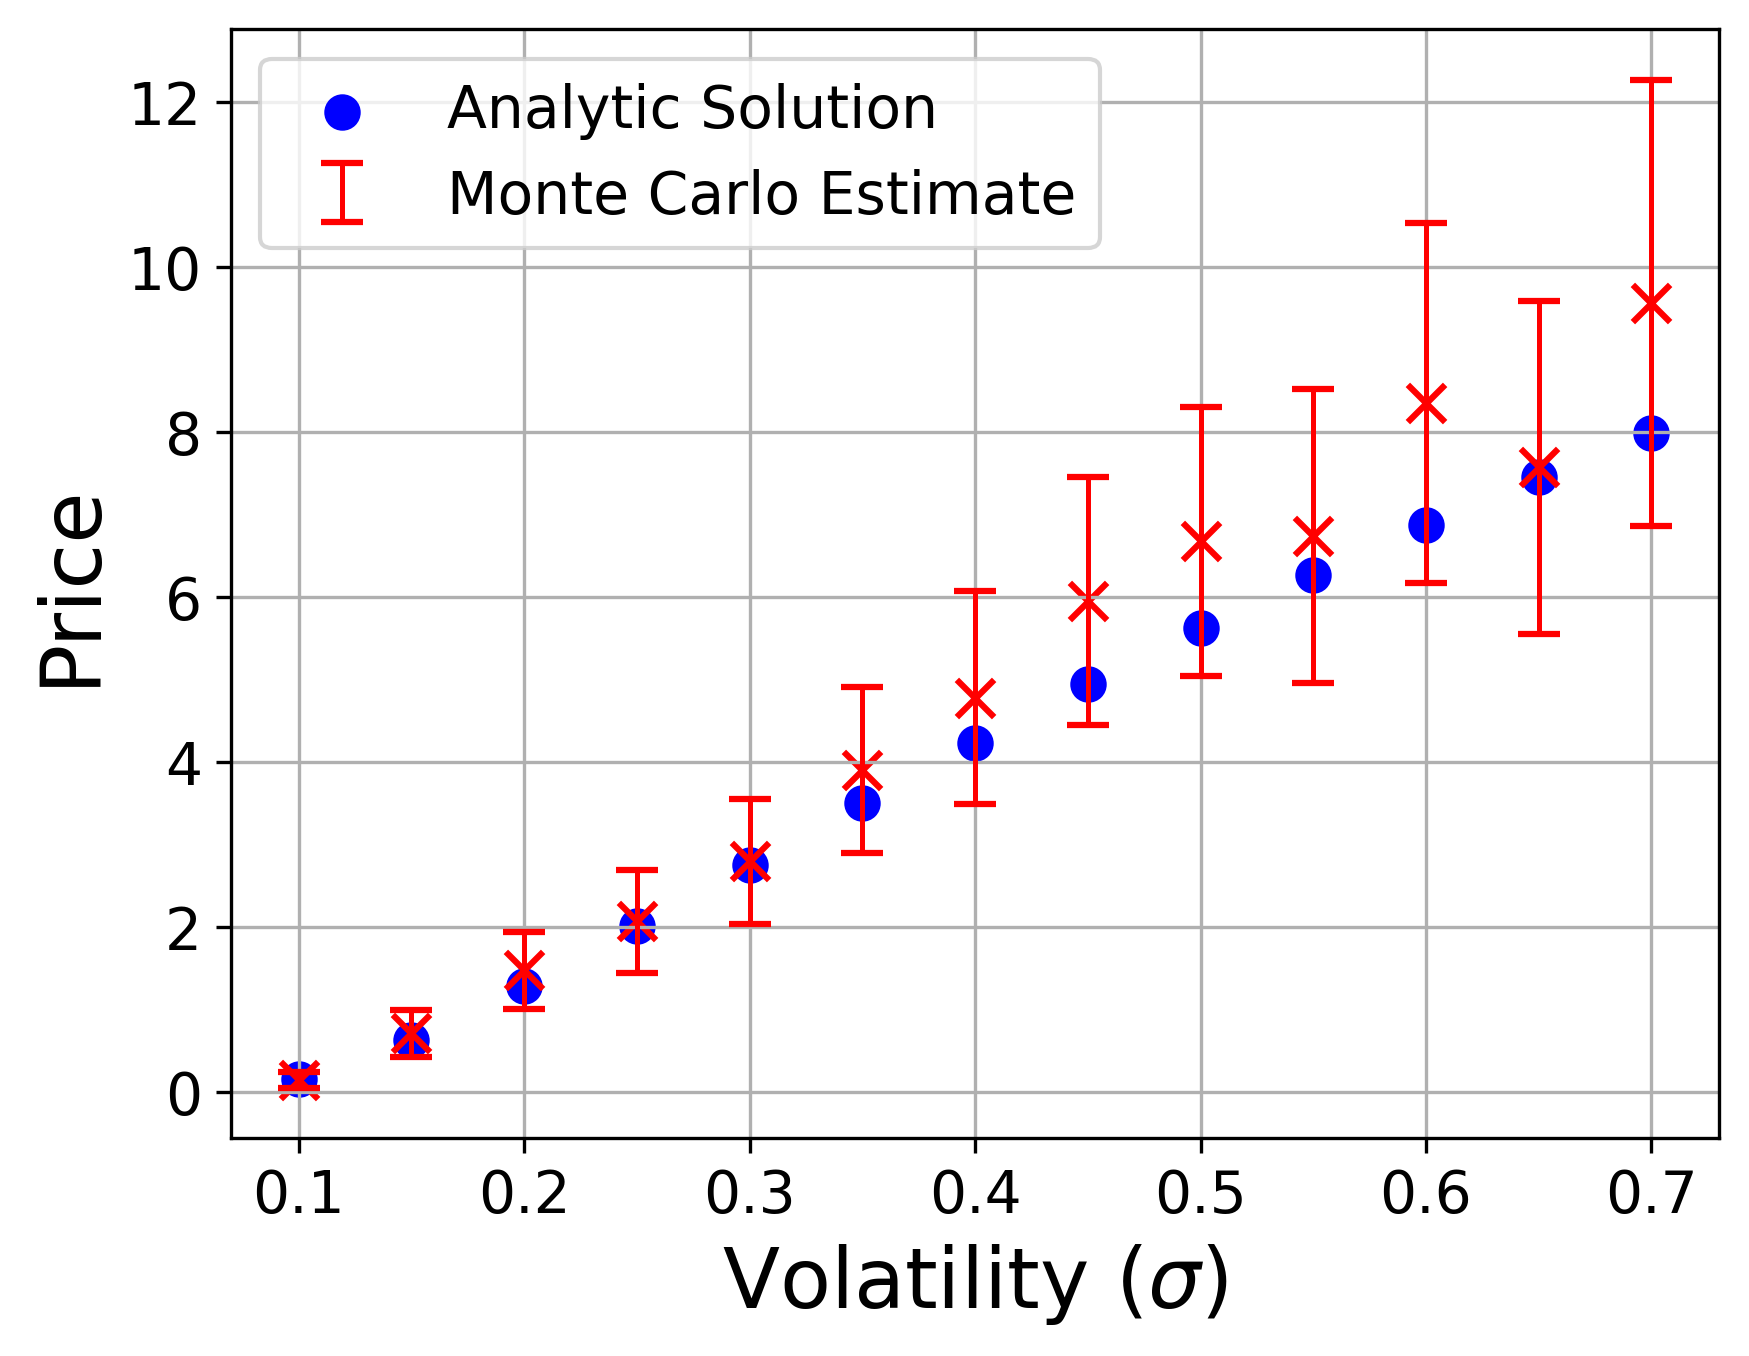
\includegraphics[width=\linewidth]{graphics/validation_mc_european_call_vol.png}
        \caption{European call prices for varying volatilities.}
        \label{fig:eu_call_vol}
    \end{subfigure}
    \hfill
    \begin{subfigure}[b]{0.45\linewidth}
        \centering
        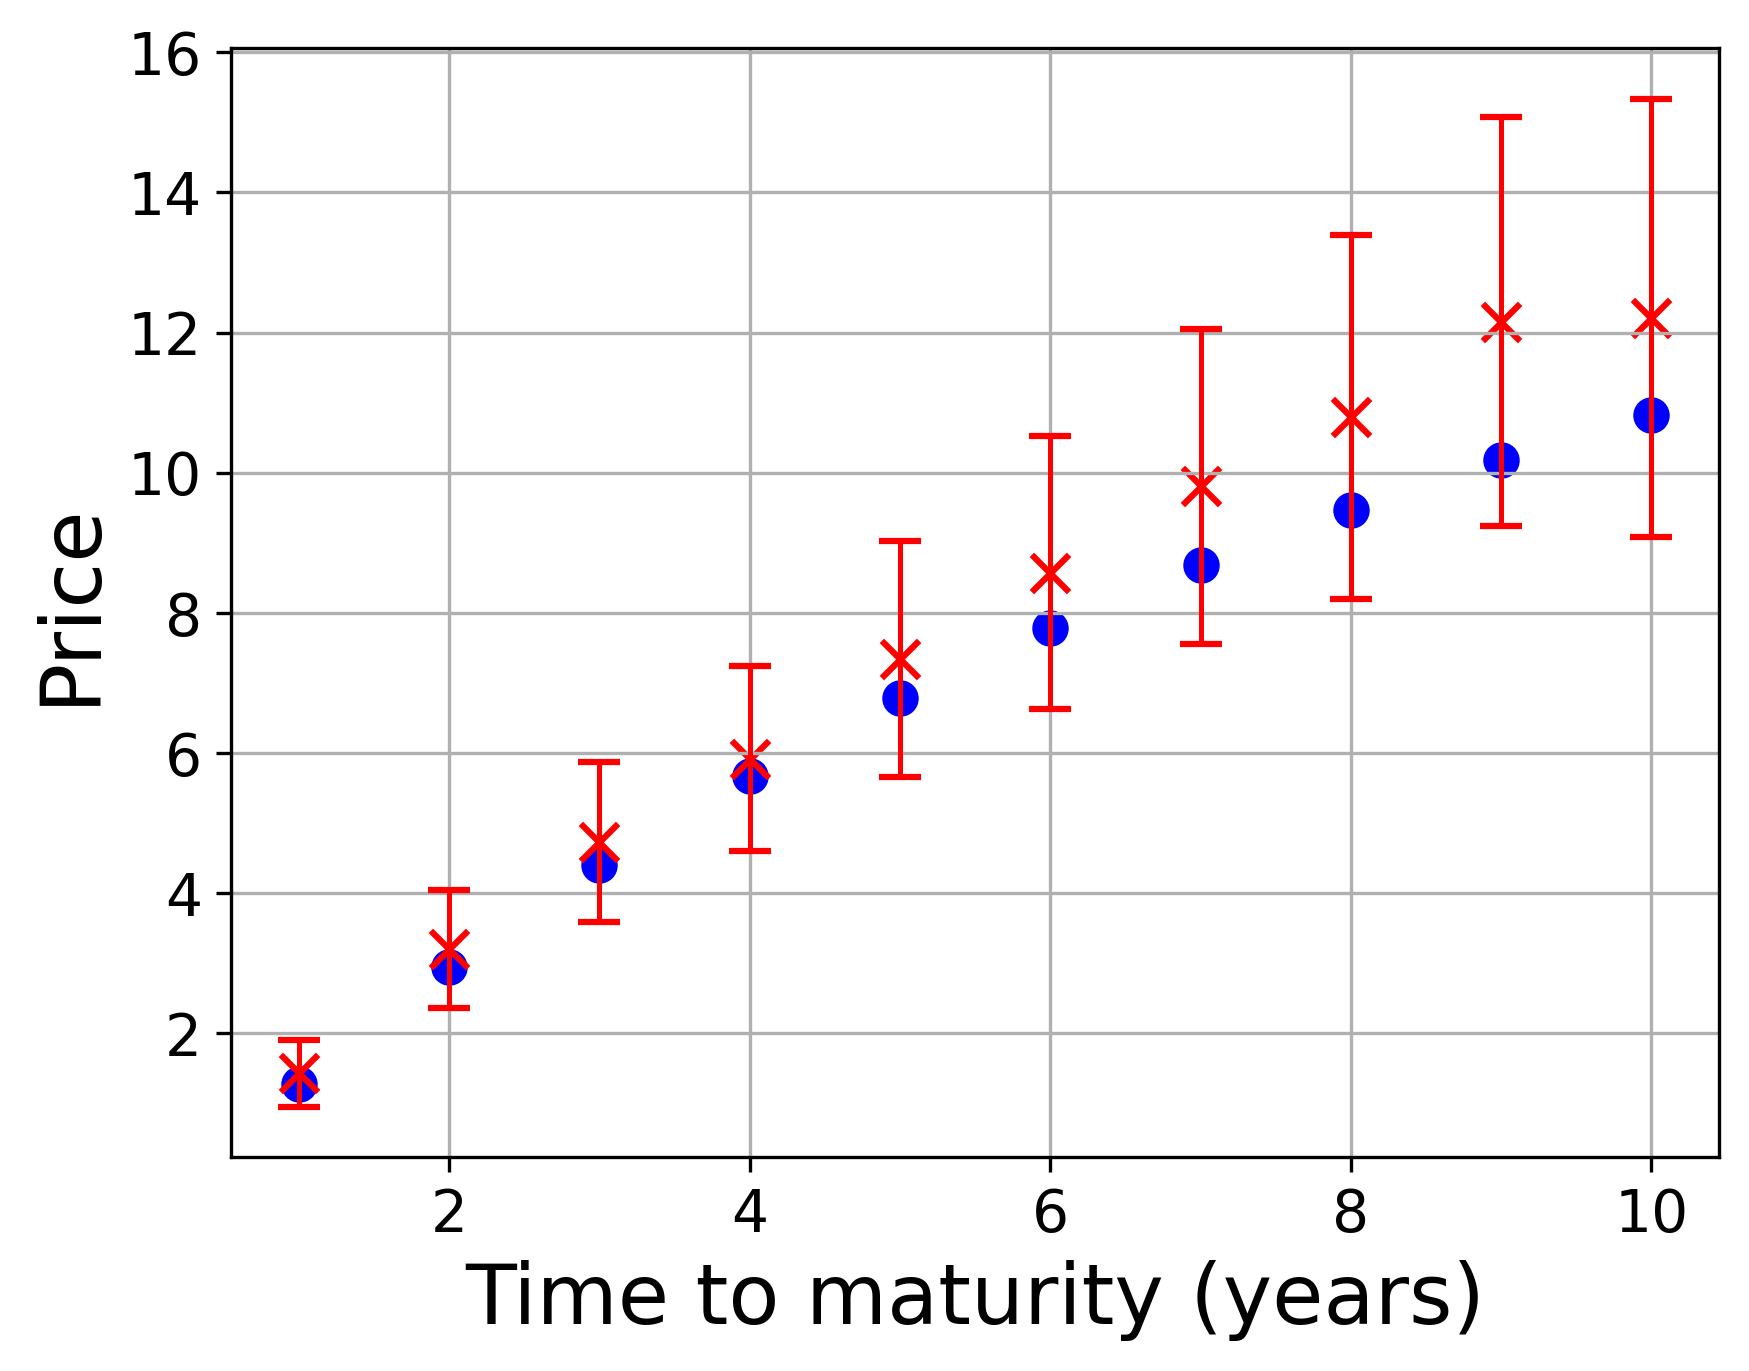
\includegraphics[width=\linewidth]{graphics/validation_mc_european_call_T.png}
        \caption{European call prices for varying maturities.}
        \label{fig:eu_call_T}
    \end{subfigure}

    \vspace{0.5cm} % Optional vertical spacing

    \begin{subfigure}[b]{0.45\linewidth}
        \centering
        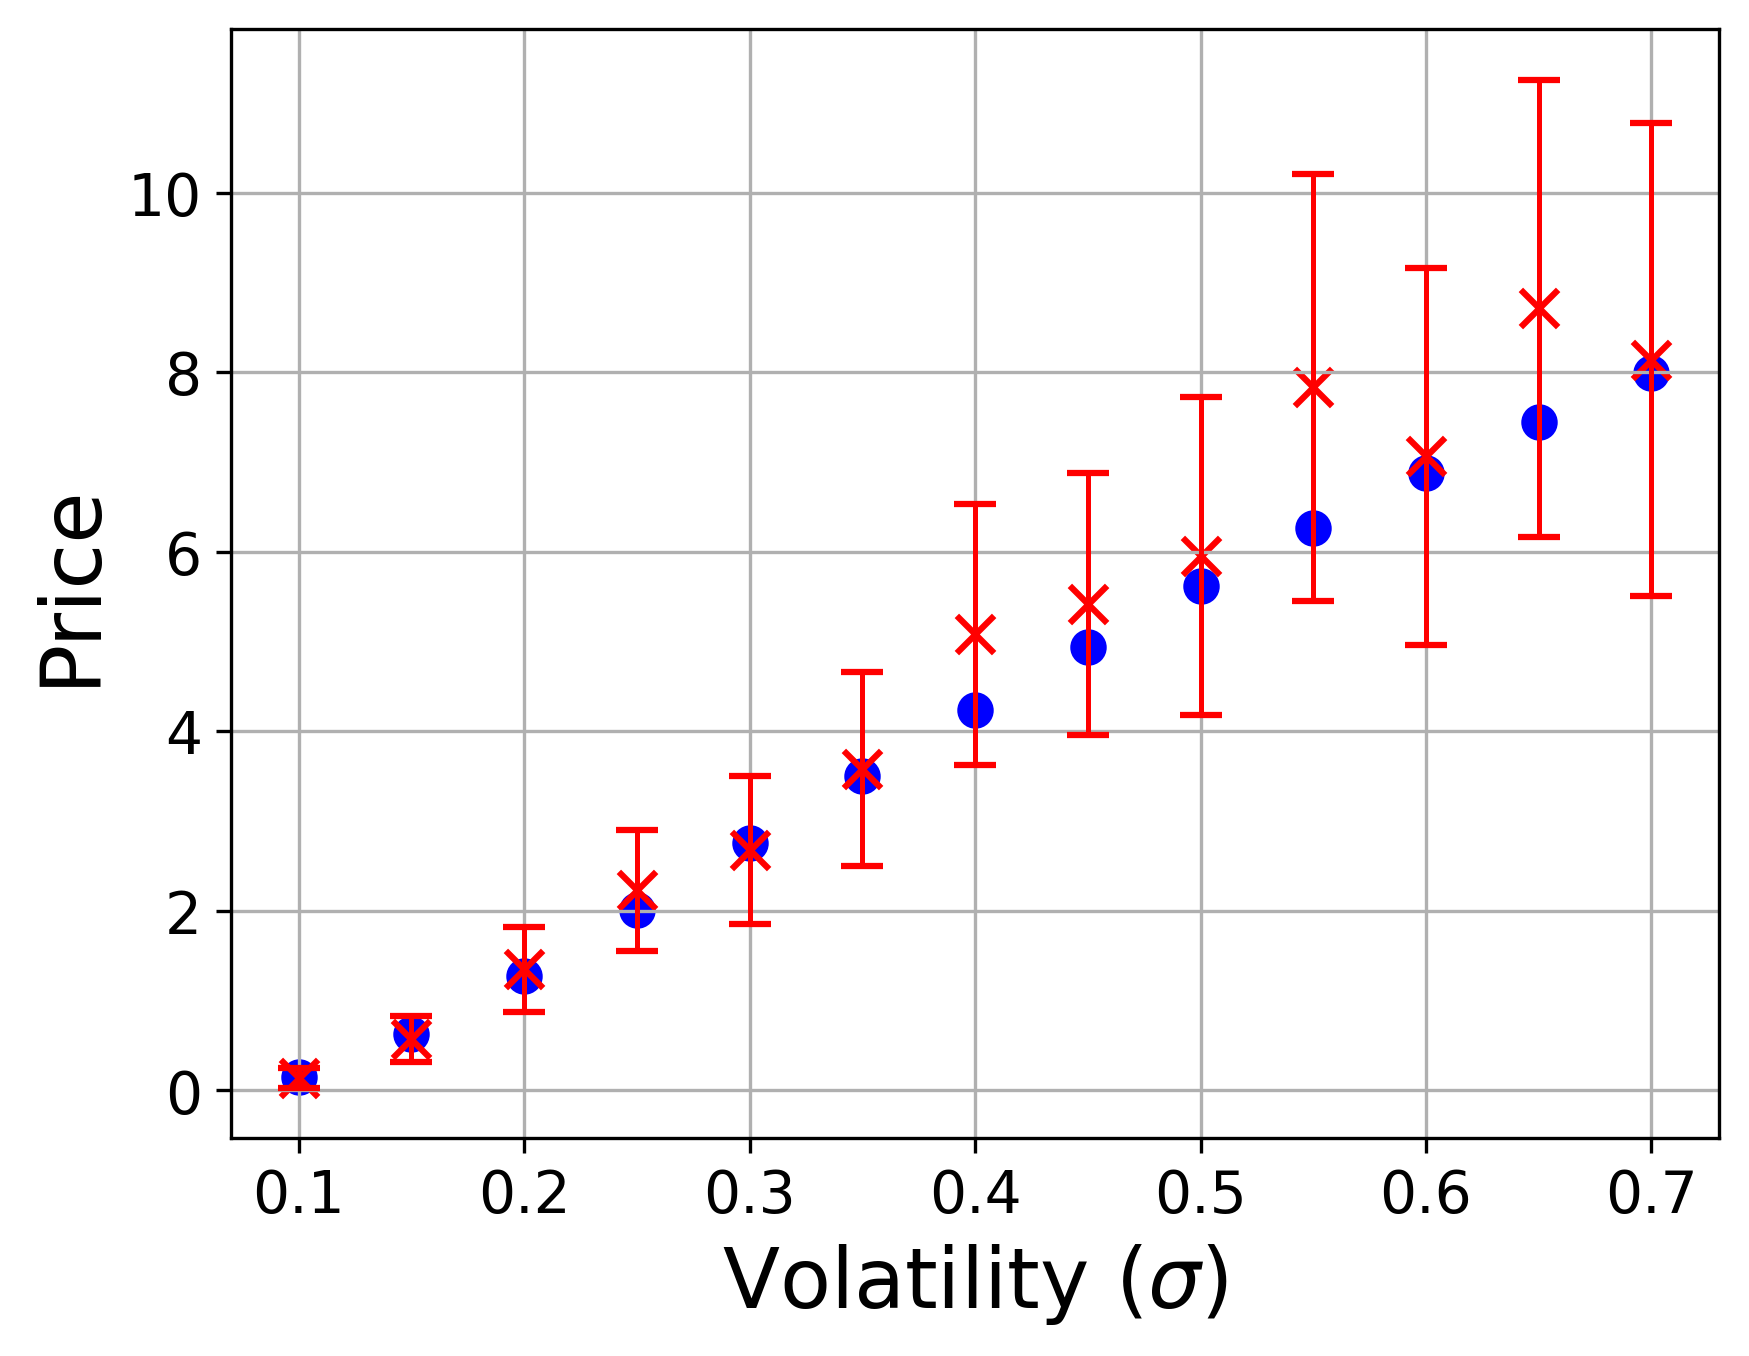
\includegraphics[width=\linewidth]{graphics/validation_mc_geometric_call_vol.png}
        \caption{Geometric Asian call prices for varying volatilities.}
        \label{fig:geometric_call_vol}
    \end{subfigure}
    \hfill
    \begin{subfigure}[b]{0.45\linewidth}
        \centering
        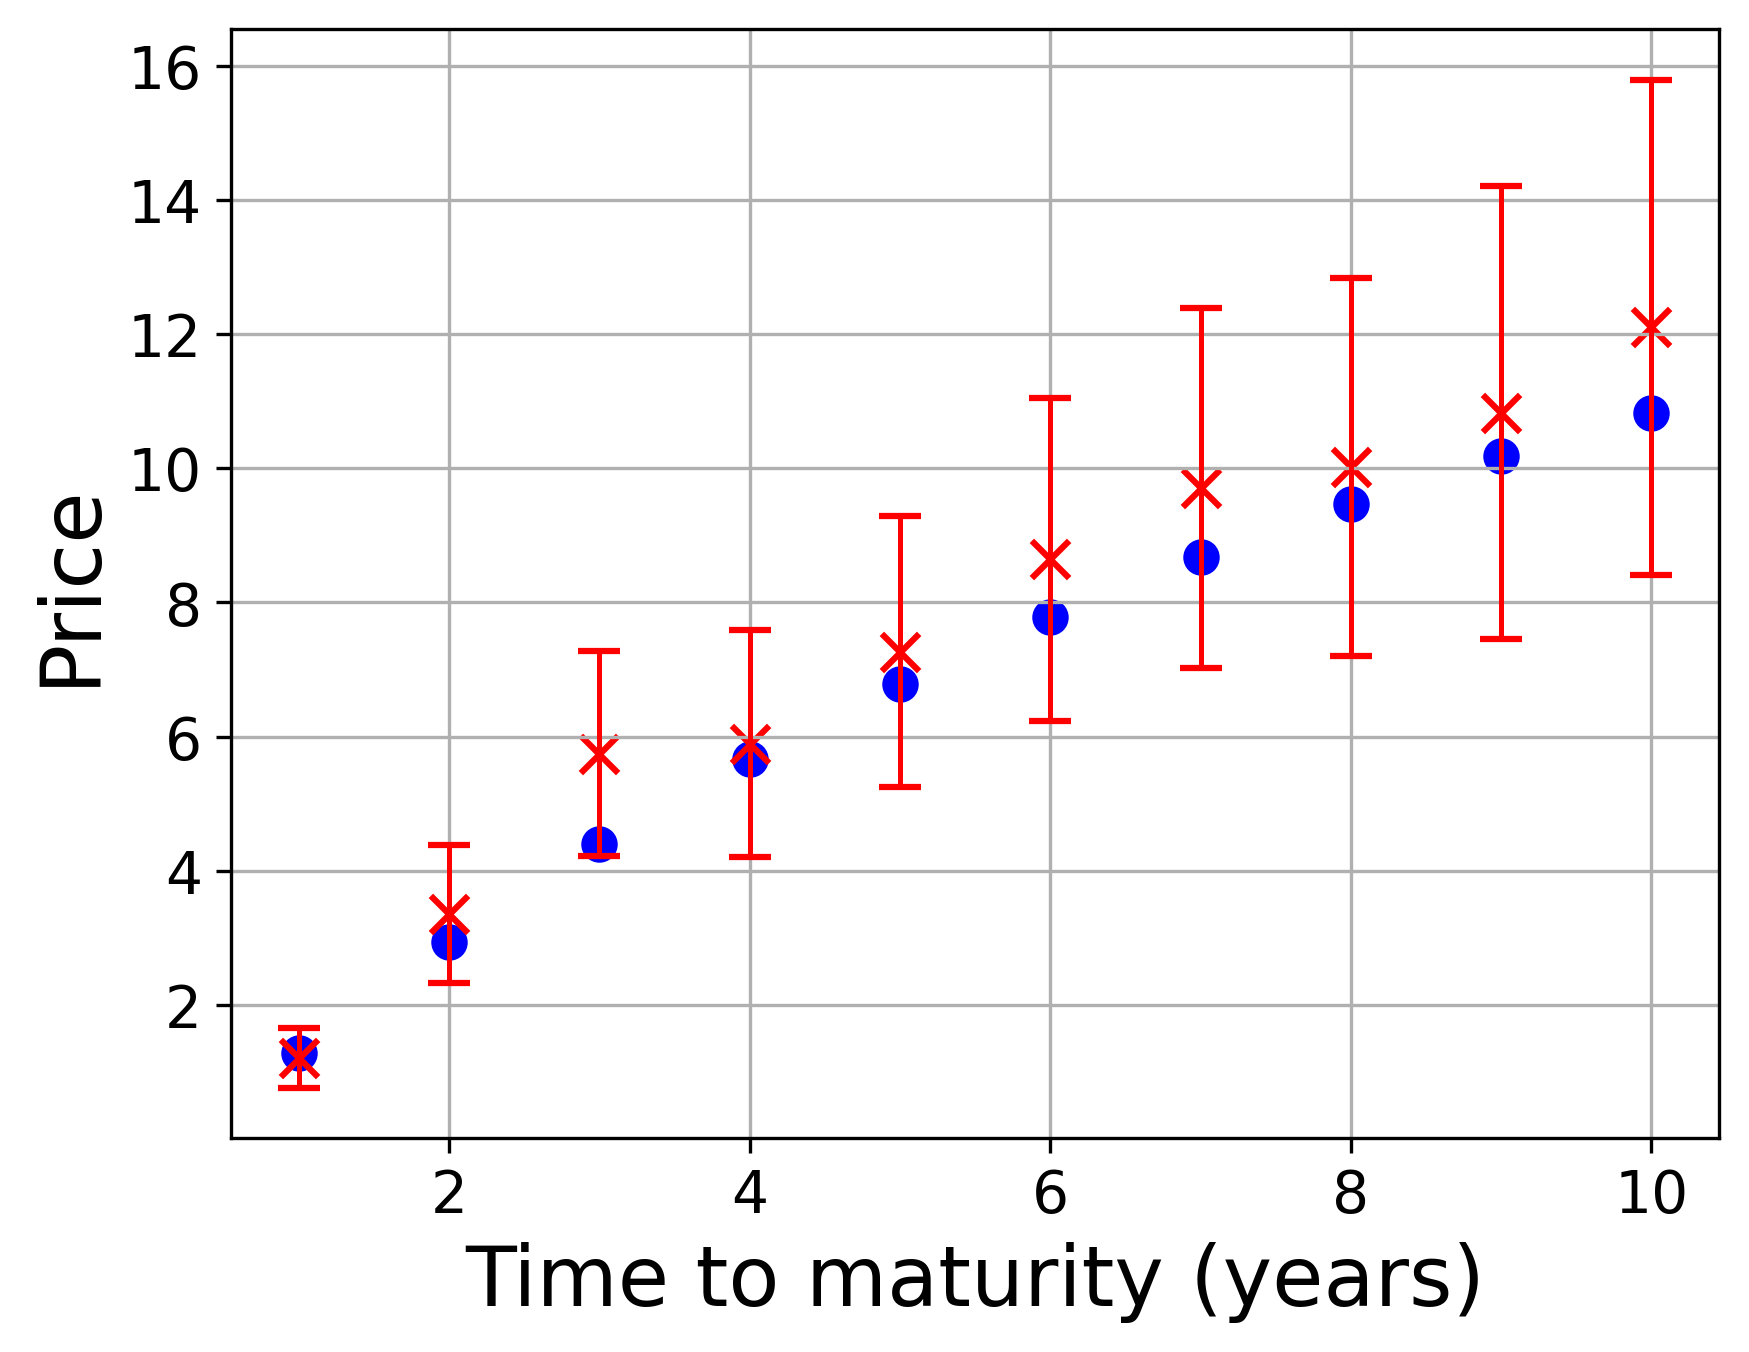
\includegraphics[width=\linewidth]{graphics/validation_mc_geometric_call_T.png}
        \caption{Geometric Asian call prices for varying maturities.}
        \label{fig:geometric_call_T}
    \end{subfigure}

    \caption{Validation of Monte Carlo pricing by comparing Monte Carlo estimates to analytic 
    solutions for European and geometric Asian call options. Prices are shown across varying 
    volatilities and maturities. Base parameters are $S_0 = 90$, $K=100$, $\sigma = 15\%$, 
    $r=4\%$, $T=1$ year, with 1000 Monte Carlo trials and timestep size 
    $\Delta T = \frac{T}{1000}$. Error bars represent the 95\% confidence intervals.}
    \label{fig:validating_MC_prices}
\end{figure}


Having validated our MC implementation, we now explore the effect of implementing
antithetic variates to achieve variance reduction. The standard Monte Carlo estimator of an 
expected payoff
$\mathbb{E}^{\mathbb{Q}}[P(S_T)]$, 
based on $M$ independent samples $S_{T,i}$ is given by:

\begin{equation*}
    \hat{\mu} = \frac{1}{M} \sum_{i=1}^{M}P(S_{T,i}).
\end{equation*}

This estimator has variance:

\begin{equation*}
    \mathrm{Var}[\hat{\mu}] = \frac{\sigma^2}{M}
\end{equation*}
where $\sigma^2 = \mathrm{Var}[P(S_{T})]$. The principle behind antithetic variates involves
 generating $\frac{M}{2}$ pairs of samples $(S_{T,i}, S_{T,i}^{anti})$, where each pair is
  constructed to exhibit negative correlation. The antithetic estimator is then defined as:

\begin{equation}
    \hat{\mu}_{anti} = \frac{1}{M/2} \sum_{i=1}^{M/2}\frac{P(S_{T,i}) + P(S_{T,i}^{anti})}{2}
\end{equation}

which is also unbiased. The variance of this estimator however is given by:

\begin{equation}
    \mathrm{Var}[\hat{\mu}_{anti}] = \frac{1}{M/2} \bigg[\frac{\mathrm{Var}[P(S_T)] + 
    \mathrm{Var}[P(S_T^{anti})] + 2\mathrm{Cov}[P(S_T), P(S_T^{anti})]}{4}\bigg].
\end{equation}

Since the pairs are negatively correlated, we have:
 $\mathrm{Cov}[P(S_T), P(S_T^{anti})] < 0$ and thus 
 $\mathrm{Var}[\hat{\mu}_{anti}] \le \mathrm{Var}[\hat{\mu}]$ indicating improved convergence.
In practice, negatively correlated samples are obtained by simulating half the underlying asset
trajectories using Brownian increments that are negatives of the other half. Figures
illustrate the resulting reduction in standard errors from employing antithetic variates.

\begin{figure}[h]
    \centering

    % First subfigure
    \begin{subfigure}[b]{0.45\linewidth}
        \centering
        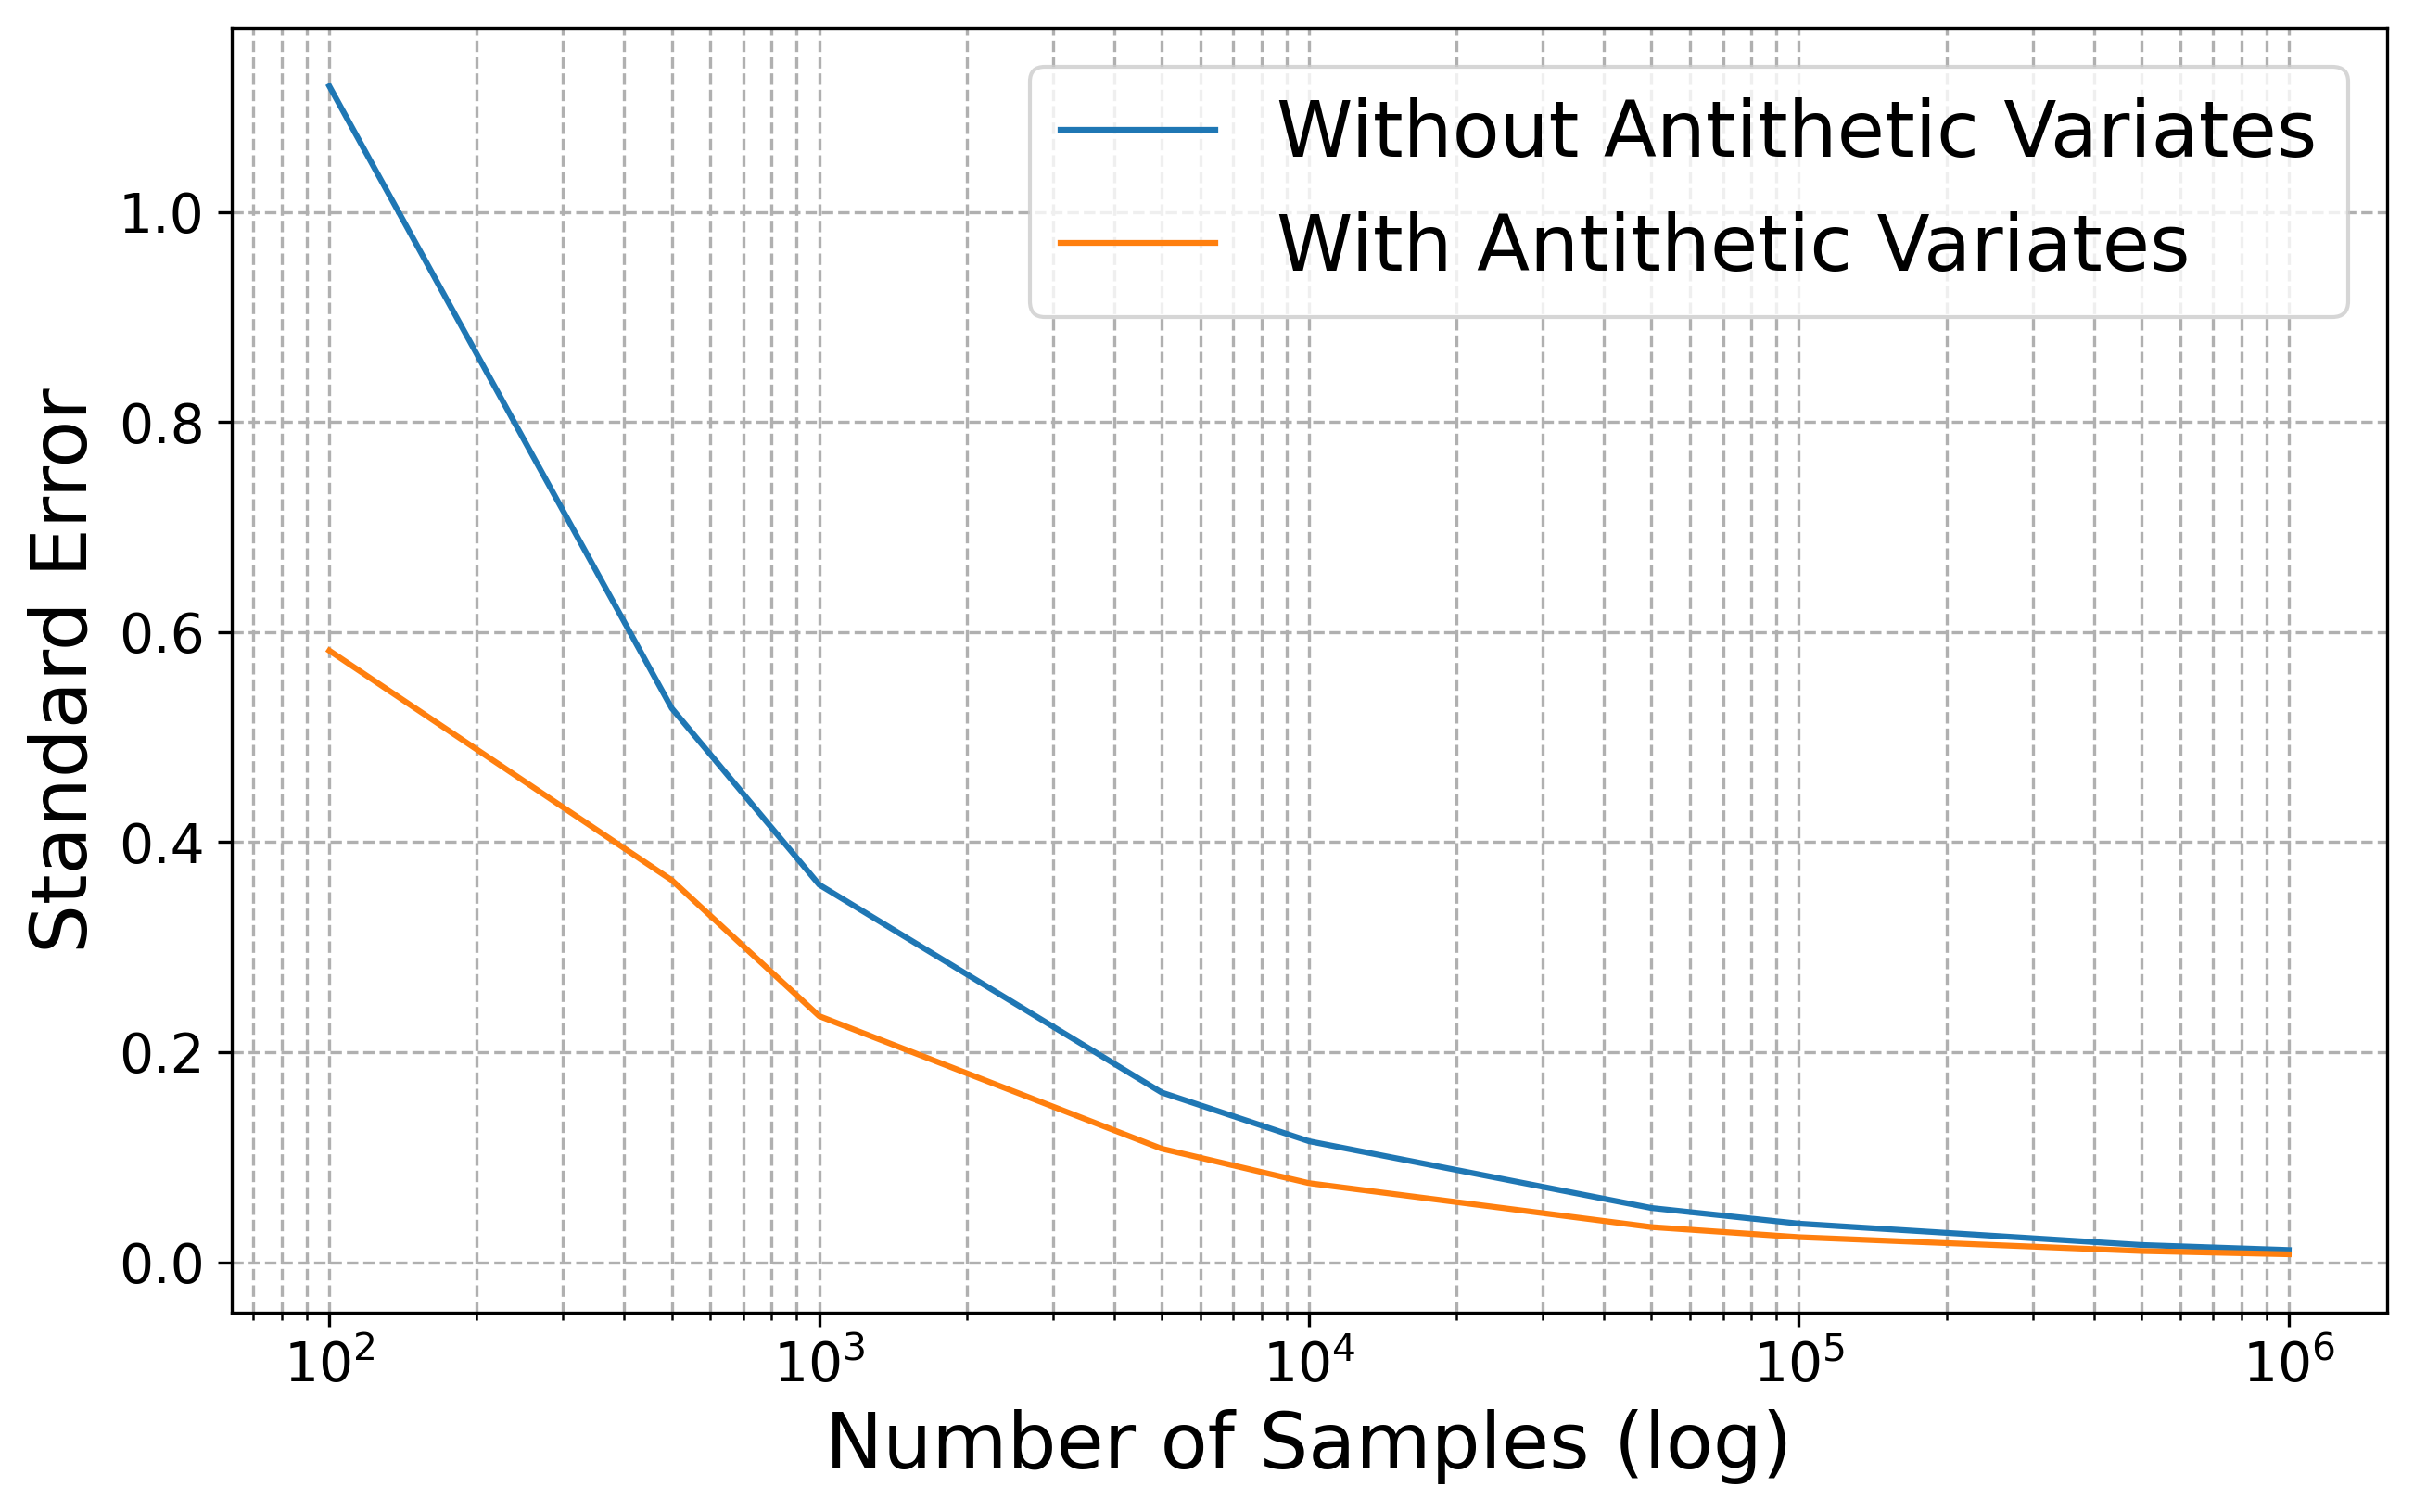
\includegraphics[width=\linewidth]{graphics/stderr_antithetic.png}
        \caption{}
        \label{fig:antithetic_vary_num_trials}
    \end{subfigure}
    \hfill
    % Second subfigure
    \begin{subfigure}[b]{0.45\linewidth}
        \centering
        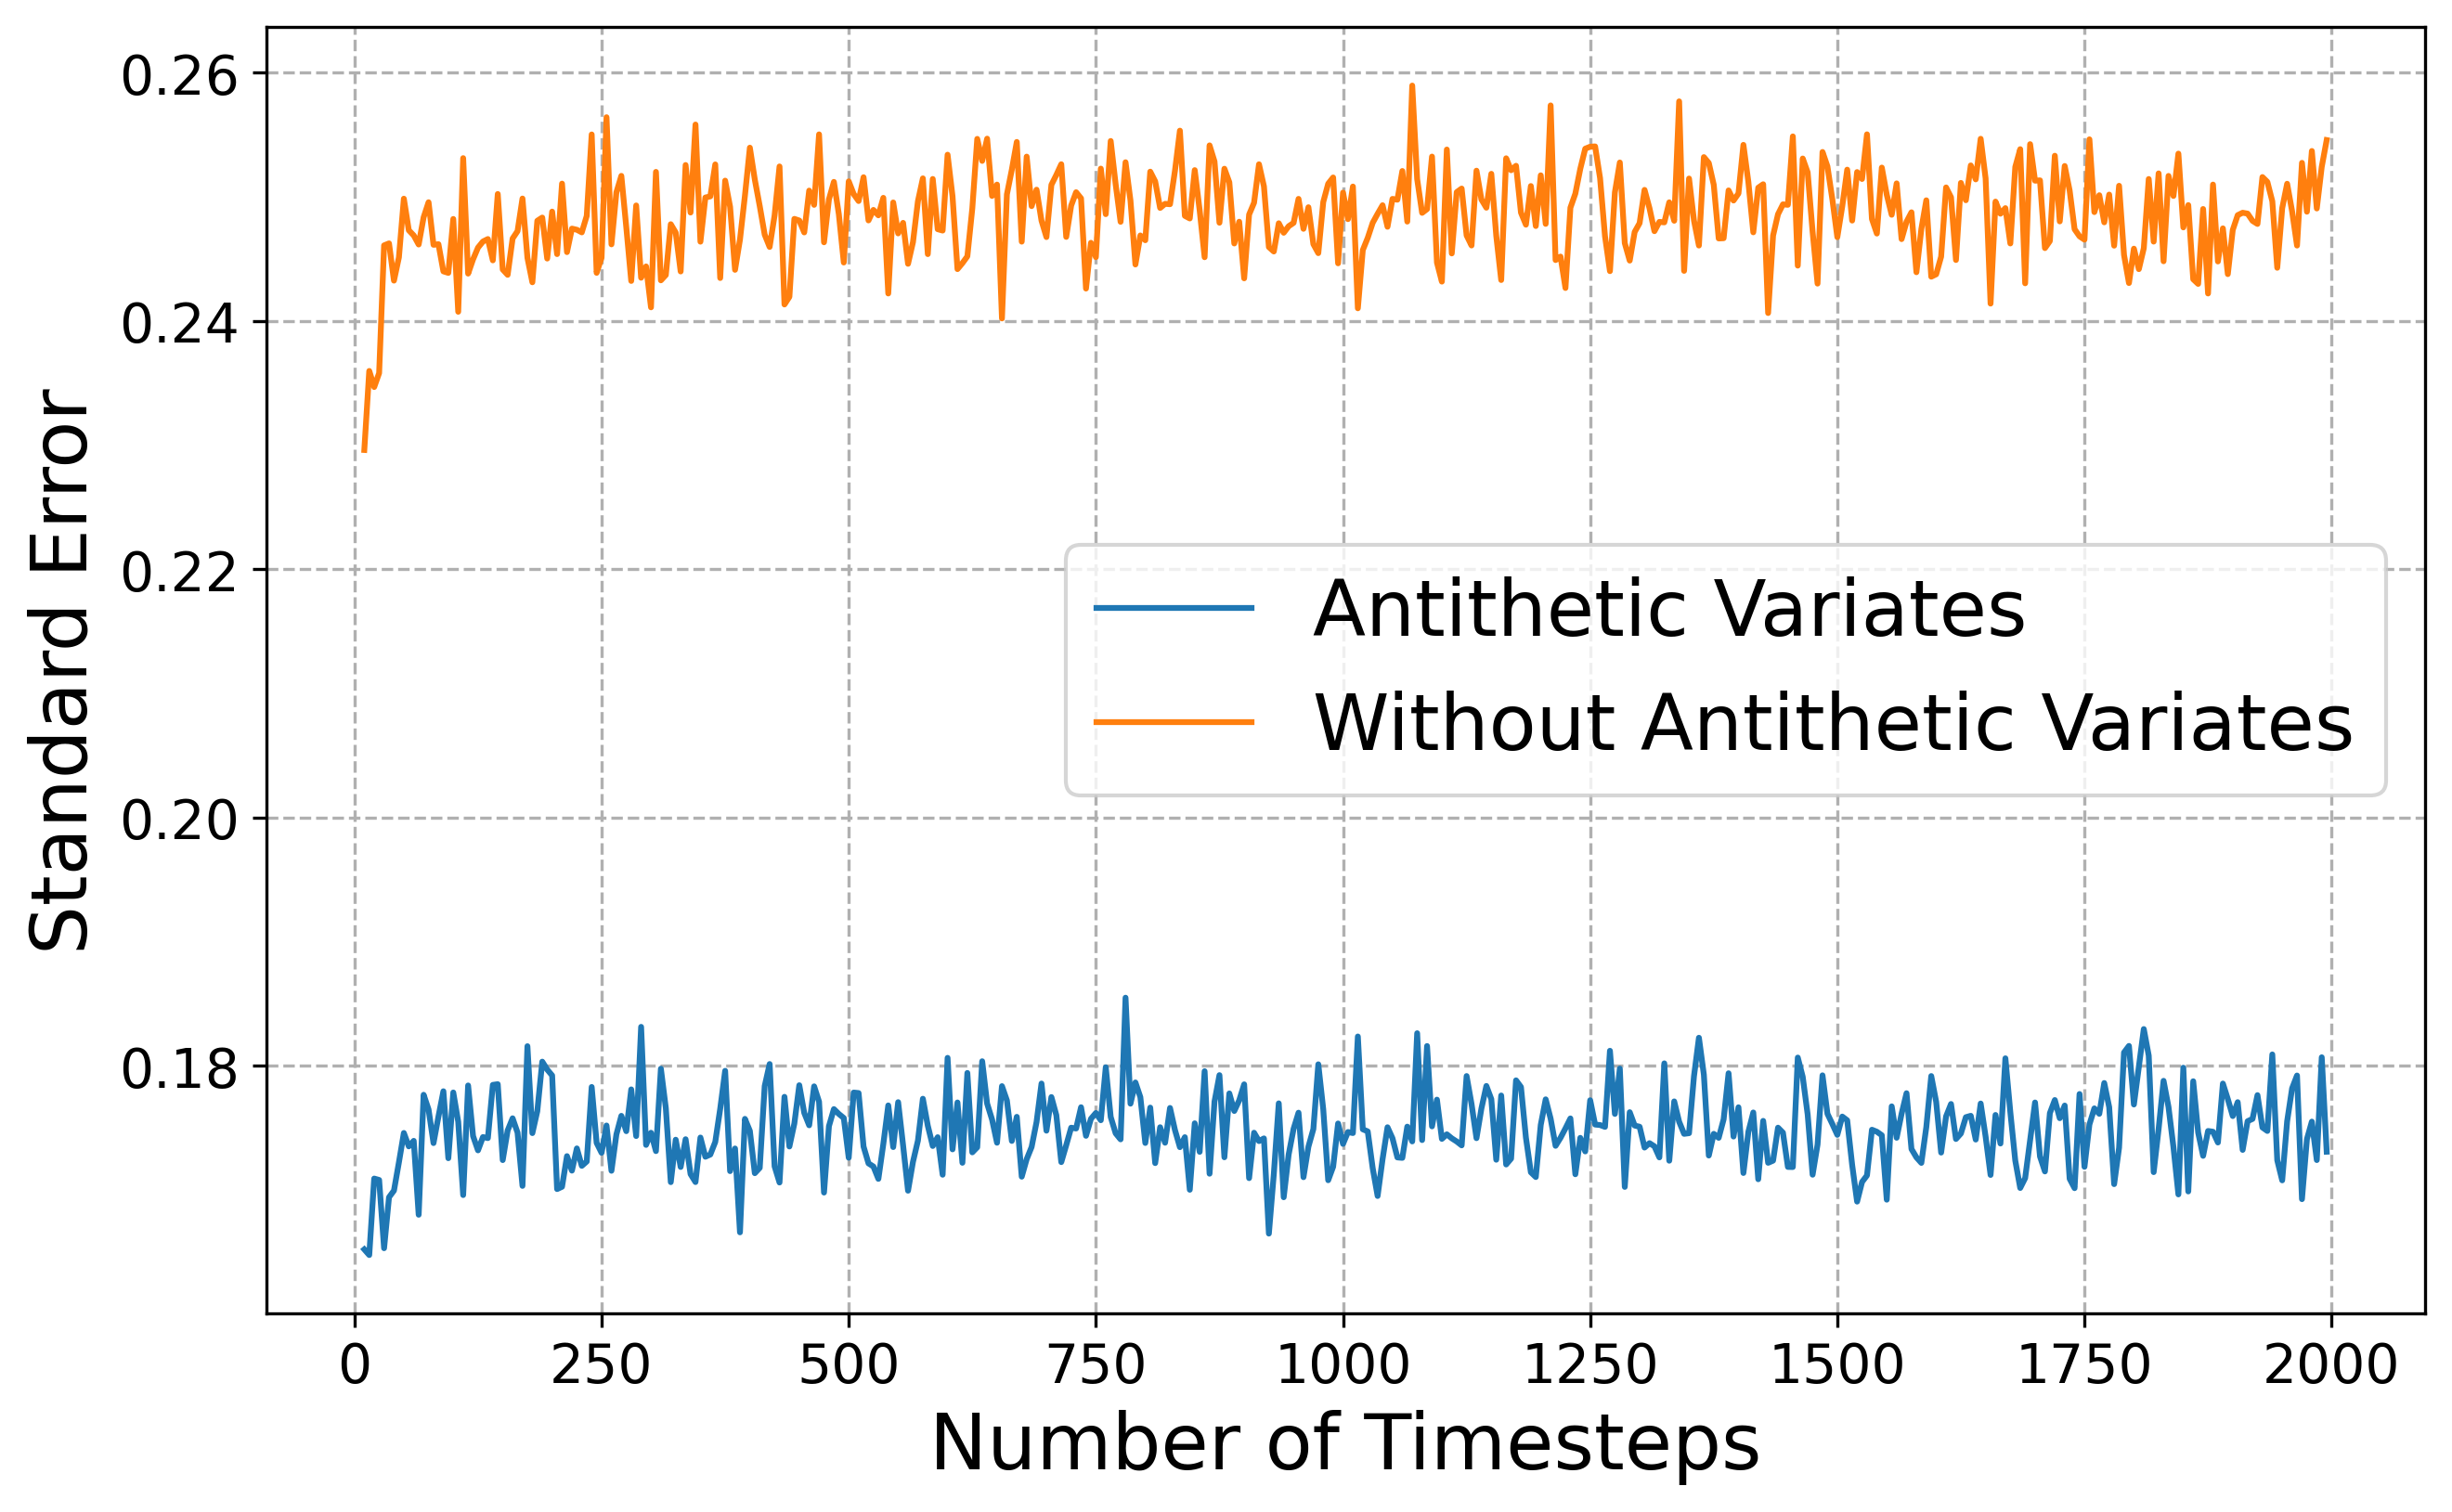
\includegraphics[width=\linewidth]{graphics/stderr_antithetic_with_n.png}
        \caption{}
        \label{fig:antithetic_vary_num_ts}
    \end{subfigure}

    \caption{Impact of using antithetic variates on Monte Carlo standard error for pricing, 
    shown when varying (a) the number of simulation samples and (b) the number of timesteps per path.
    Results were generated using the same base parameters as in Figure \ref{fig:validating_MC_prices} 
    for a European call.}
    \label{fig:std_errors_antithetic_compared}
\end{figure}

We observe a clear reduction in the standard error, 
resulting in faster convergence of Monte Carlo estimates when employing antithetic variates. 
Having validated the effectiveness of antithetic variates, we now proceed to implement this technique 
in pricing arithmetic Asian options. Subsequently, we will explore an additional variance reduction 
strategy, the control variate method, which we expect will further enhance the efficiency and accuracy 
of our Monte Carlo pricing framework.

\subsection{Pricing arithmetic Asian options}

Obtaining prices for arithmetic Asian options is simply now a case of changing the payoff function 
used to that described by equations \eqref{eq:asian_payoffs}. We now plot the obtained prices for 
arithmetic Asian put and call options for varying varying strikes and volatilities alongside now
validated prices for European and geometric Asian options. Results are shown in Figure 
\ref{fig:asian_arith_prices}


\begin{figure}[h]
    \centering
% Top left
\begin{subfigure}[b]{0.45\linewidth}
    \centering
    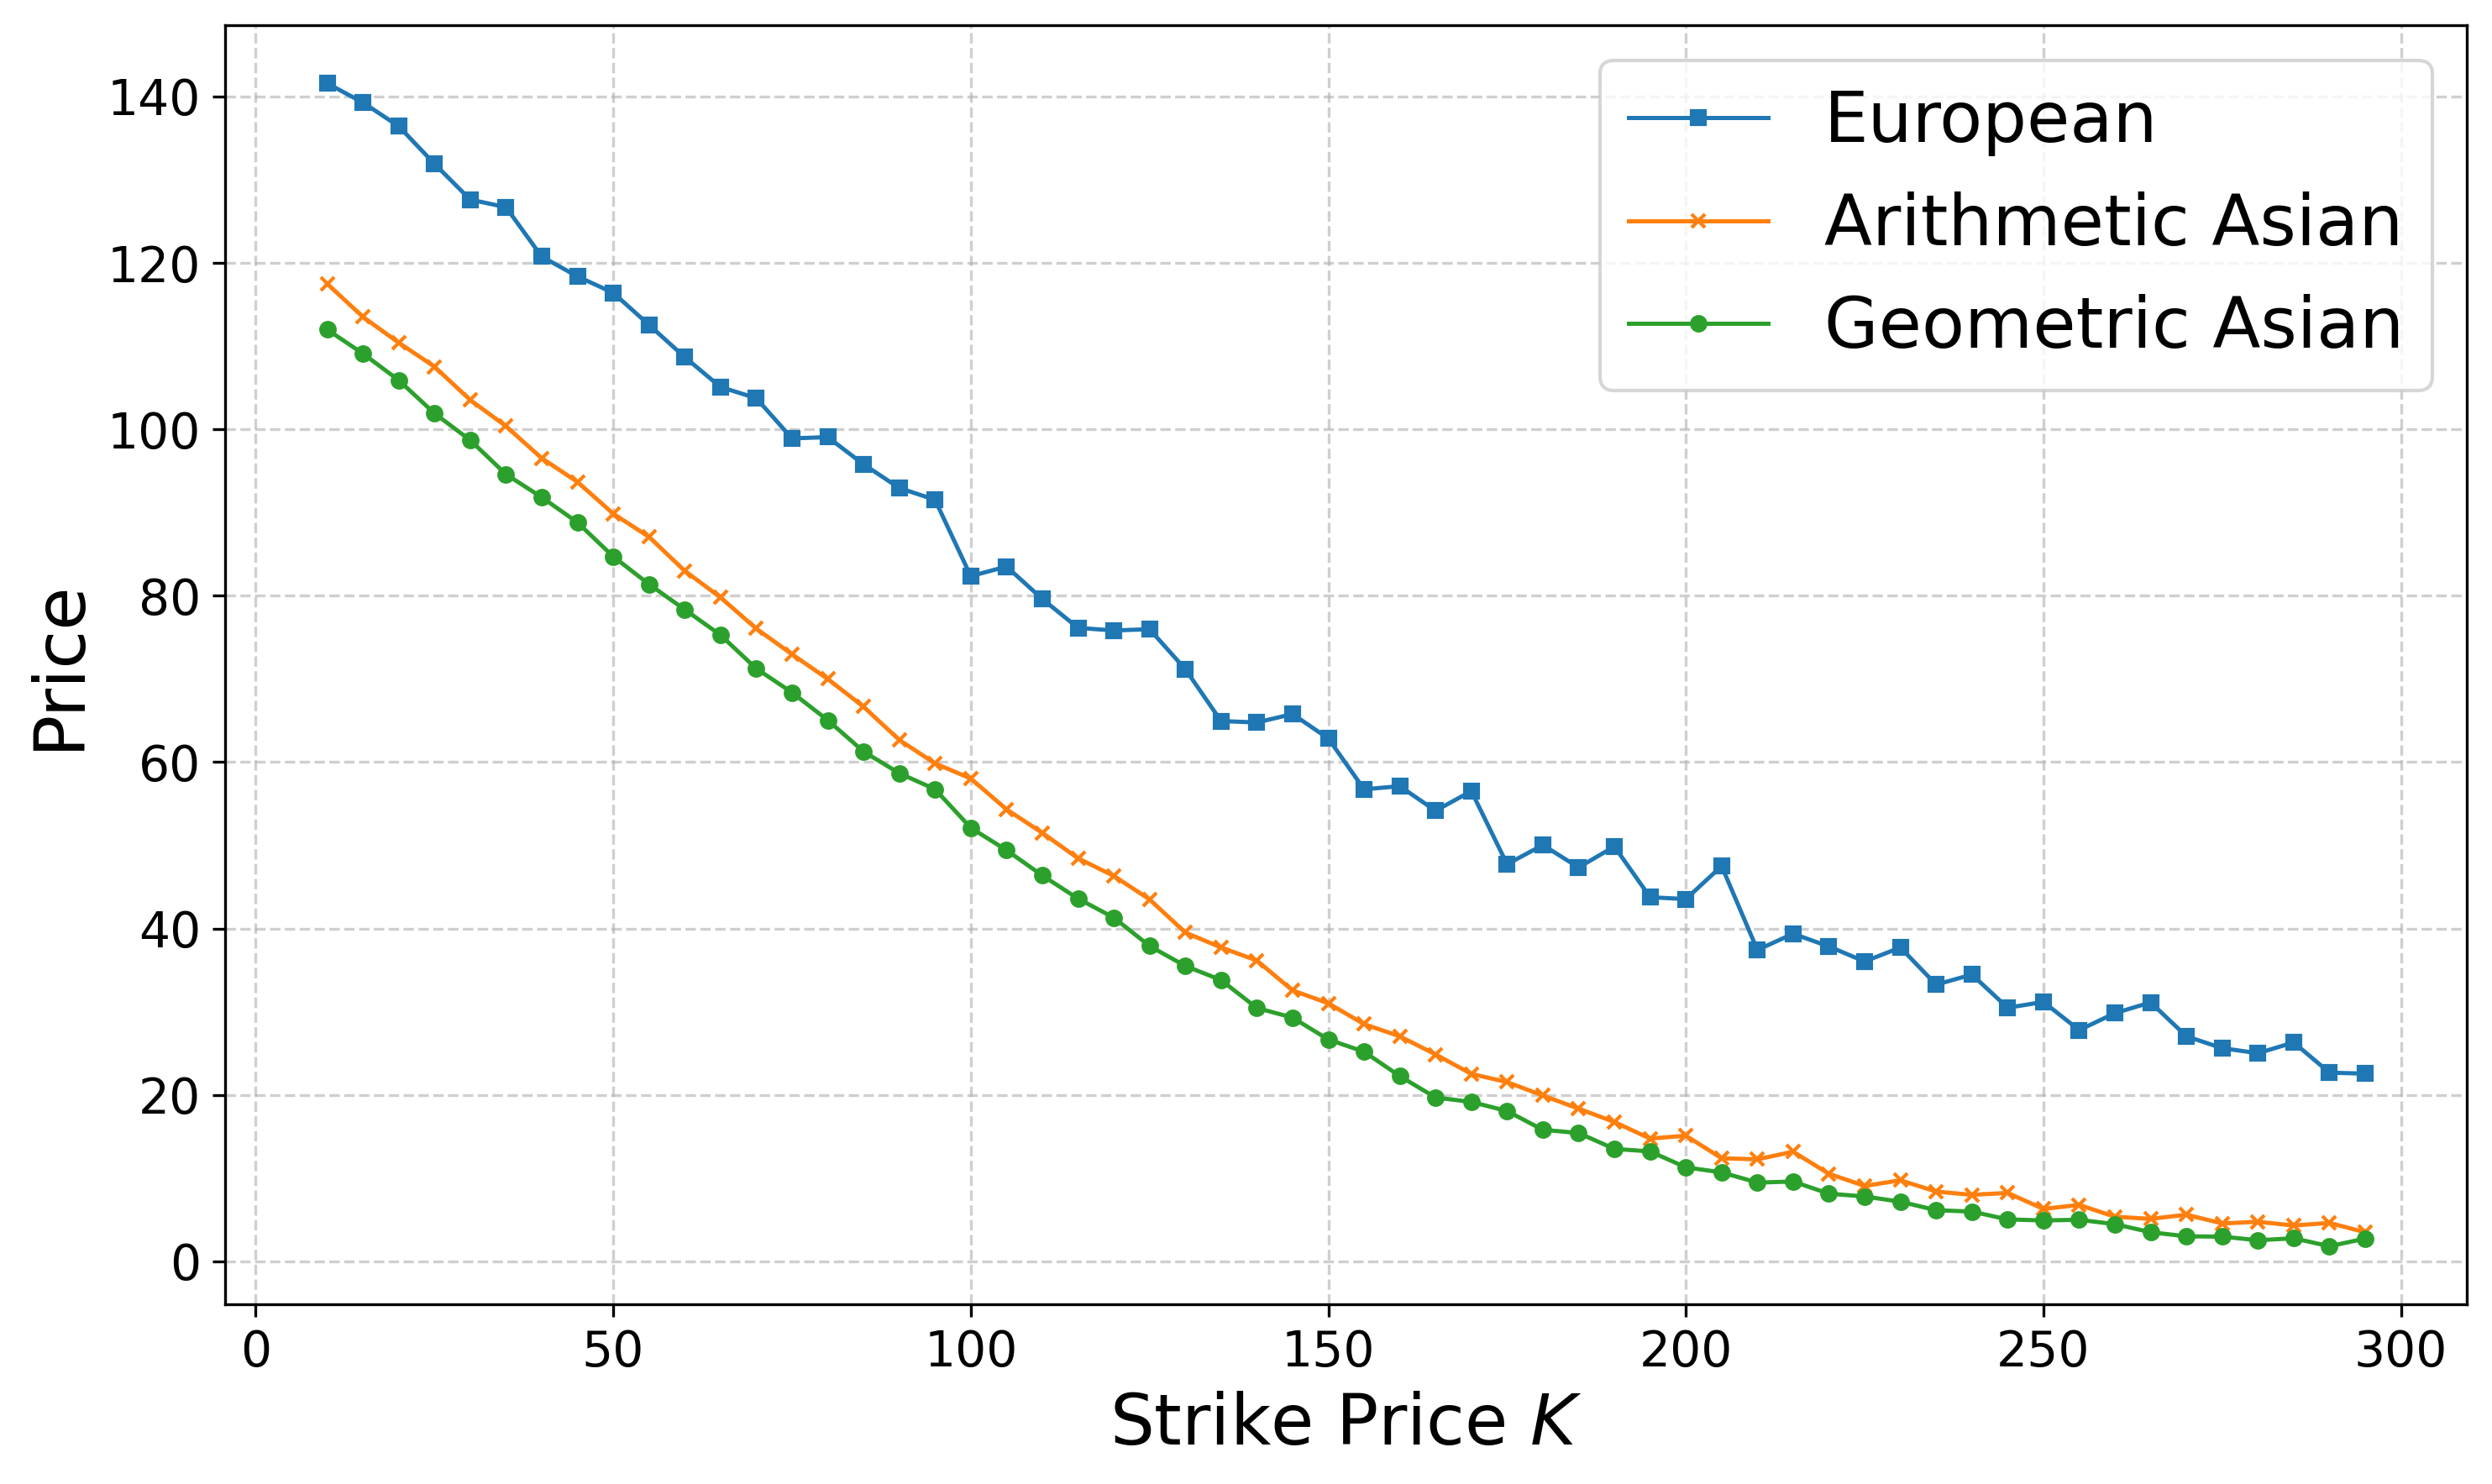
\includegraphics[width=\linewidth]{graphics/arithmetic_call_prices_K.png}
    \caption{Call option prices varying strike $K$.}
    \label{fig:arith_call_k}
\end{subfigure}
\hfill
% Top right
\begin{subfigure}[b]{0.45\linewidth}
    \centering
    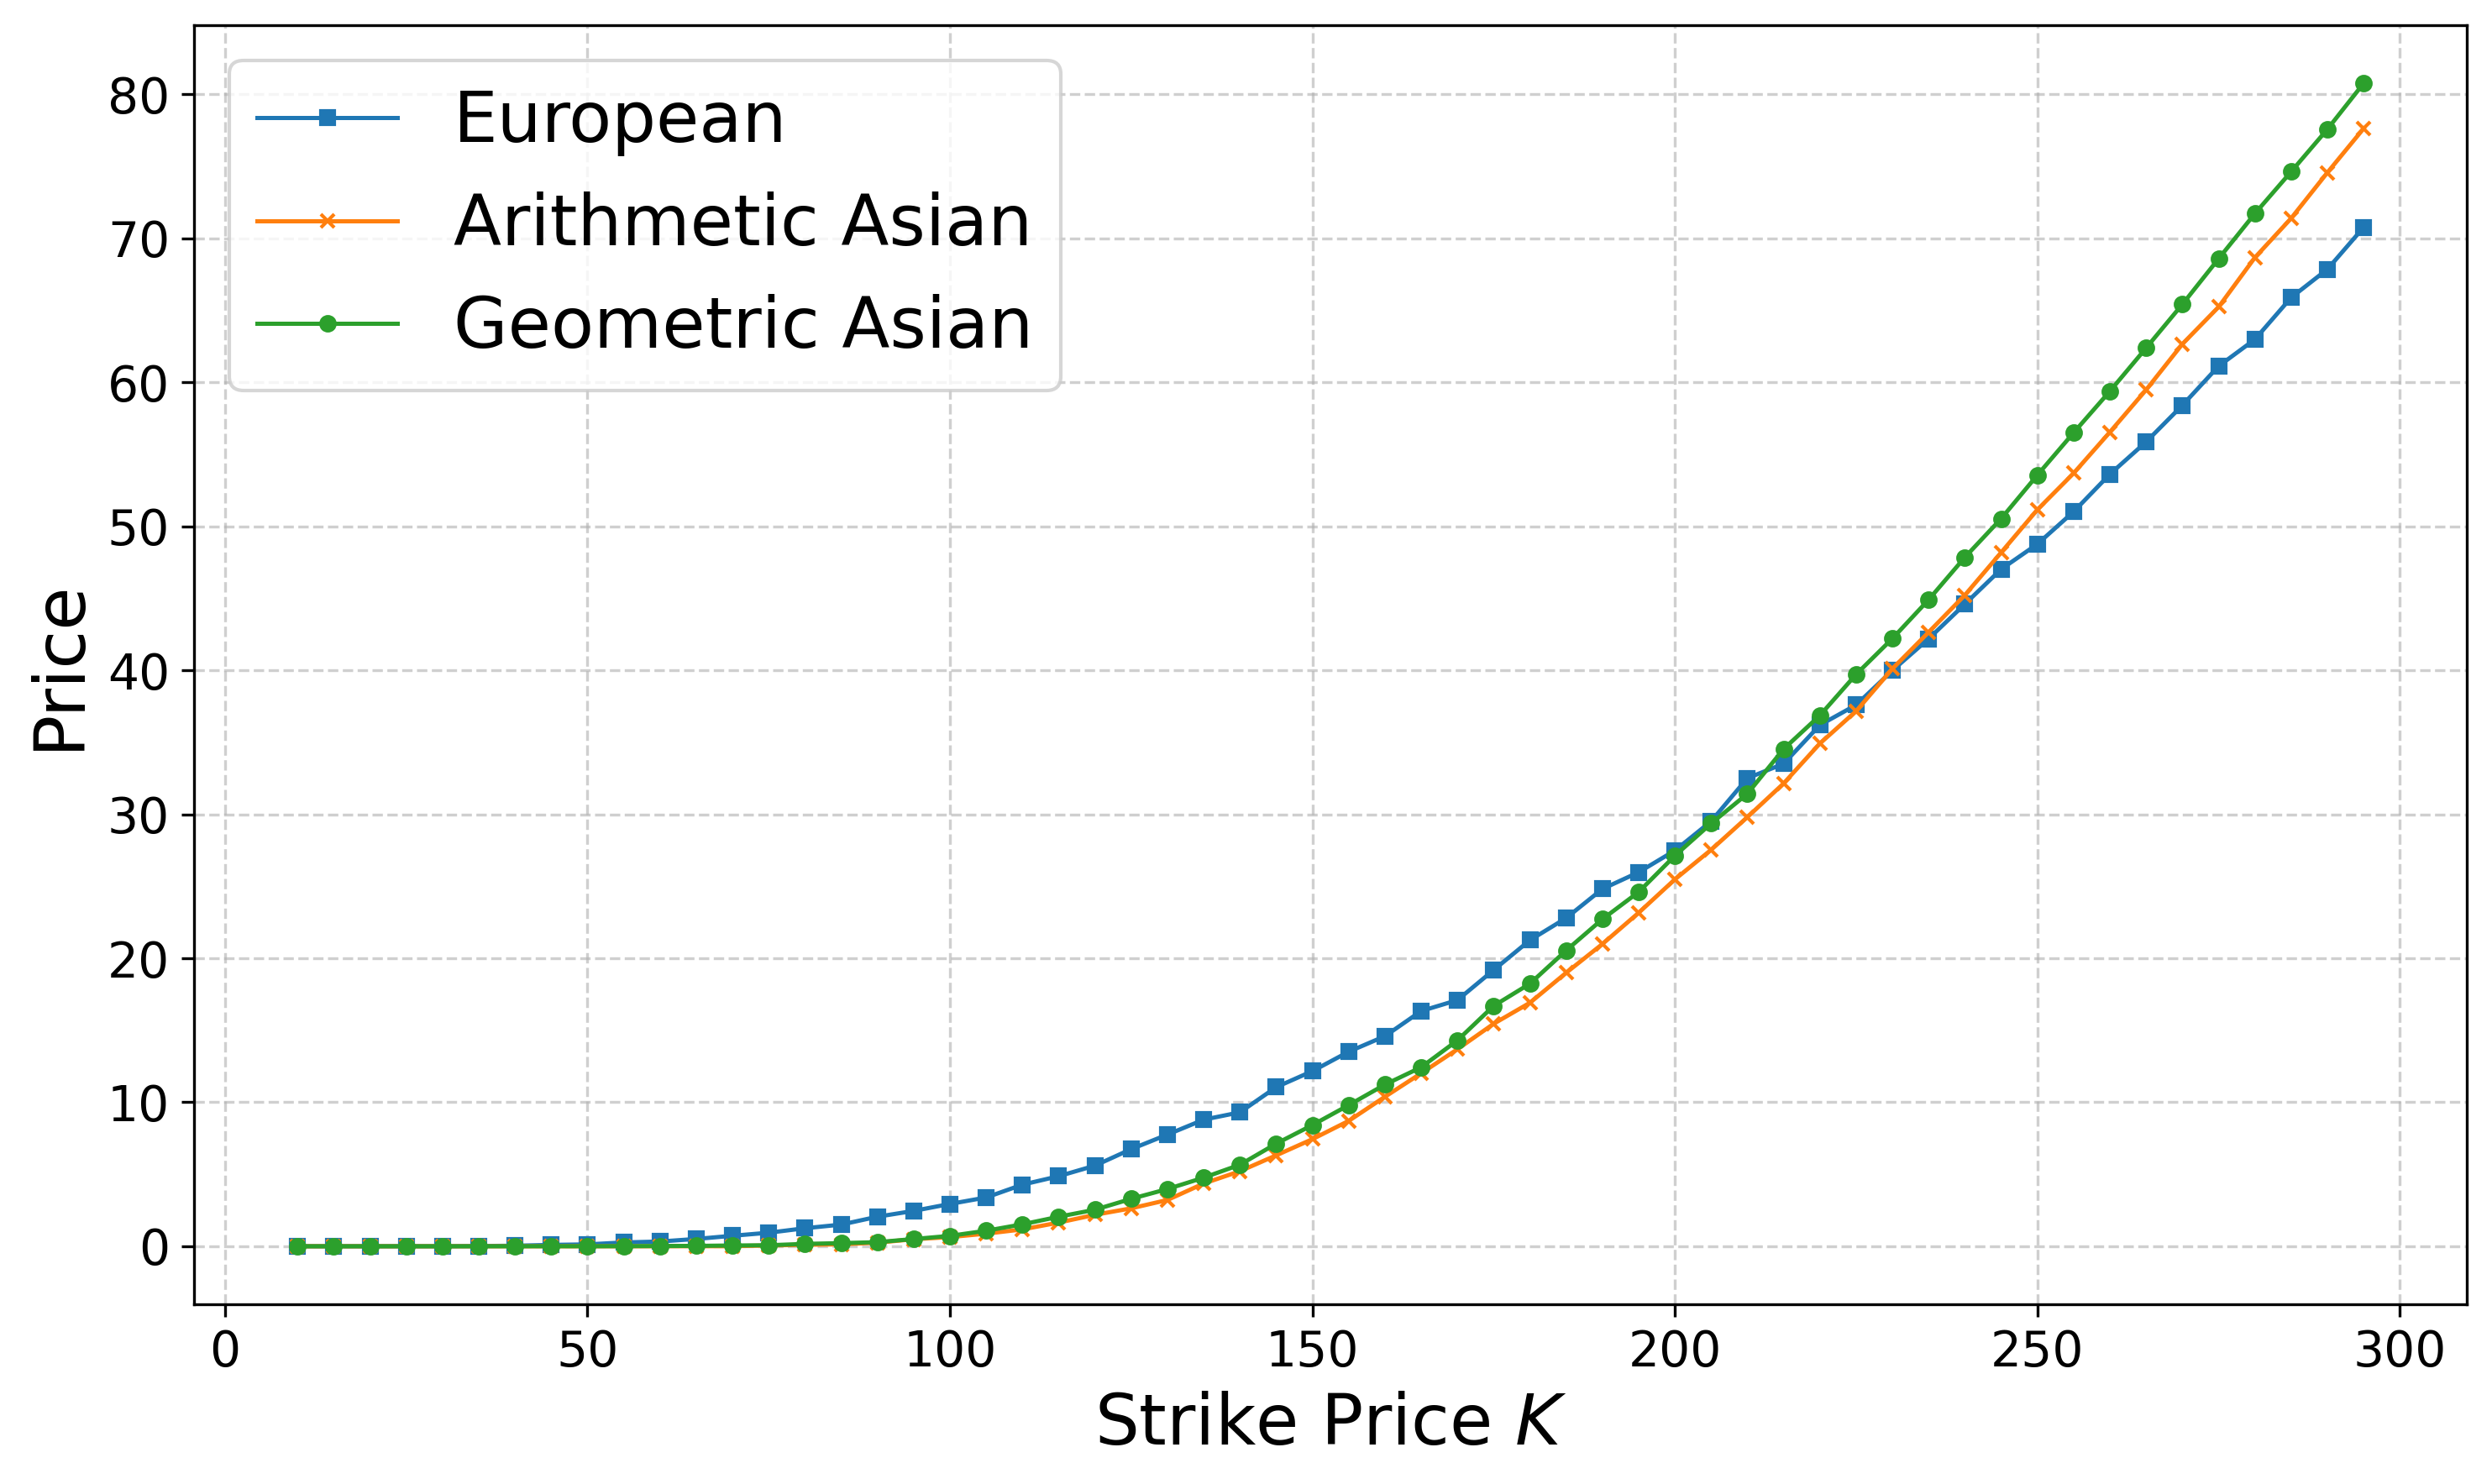
\includegraphics[width=\linewidth]{graphics/arithmetic_put_prices_K.png}
    \caption{Put option prices varying strike $K$.}
    \label{fig:arith_put_k}
\end{subfigure}

\vspace{0.5cm}

% Bottom left
\begin{subfigure}[b]{0.45\linewidth}
    \centering
    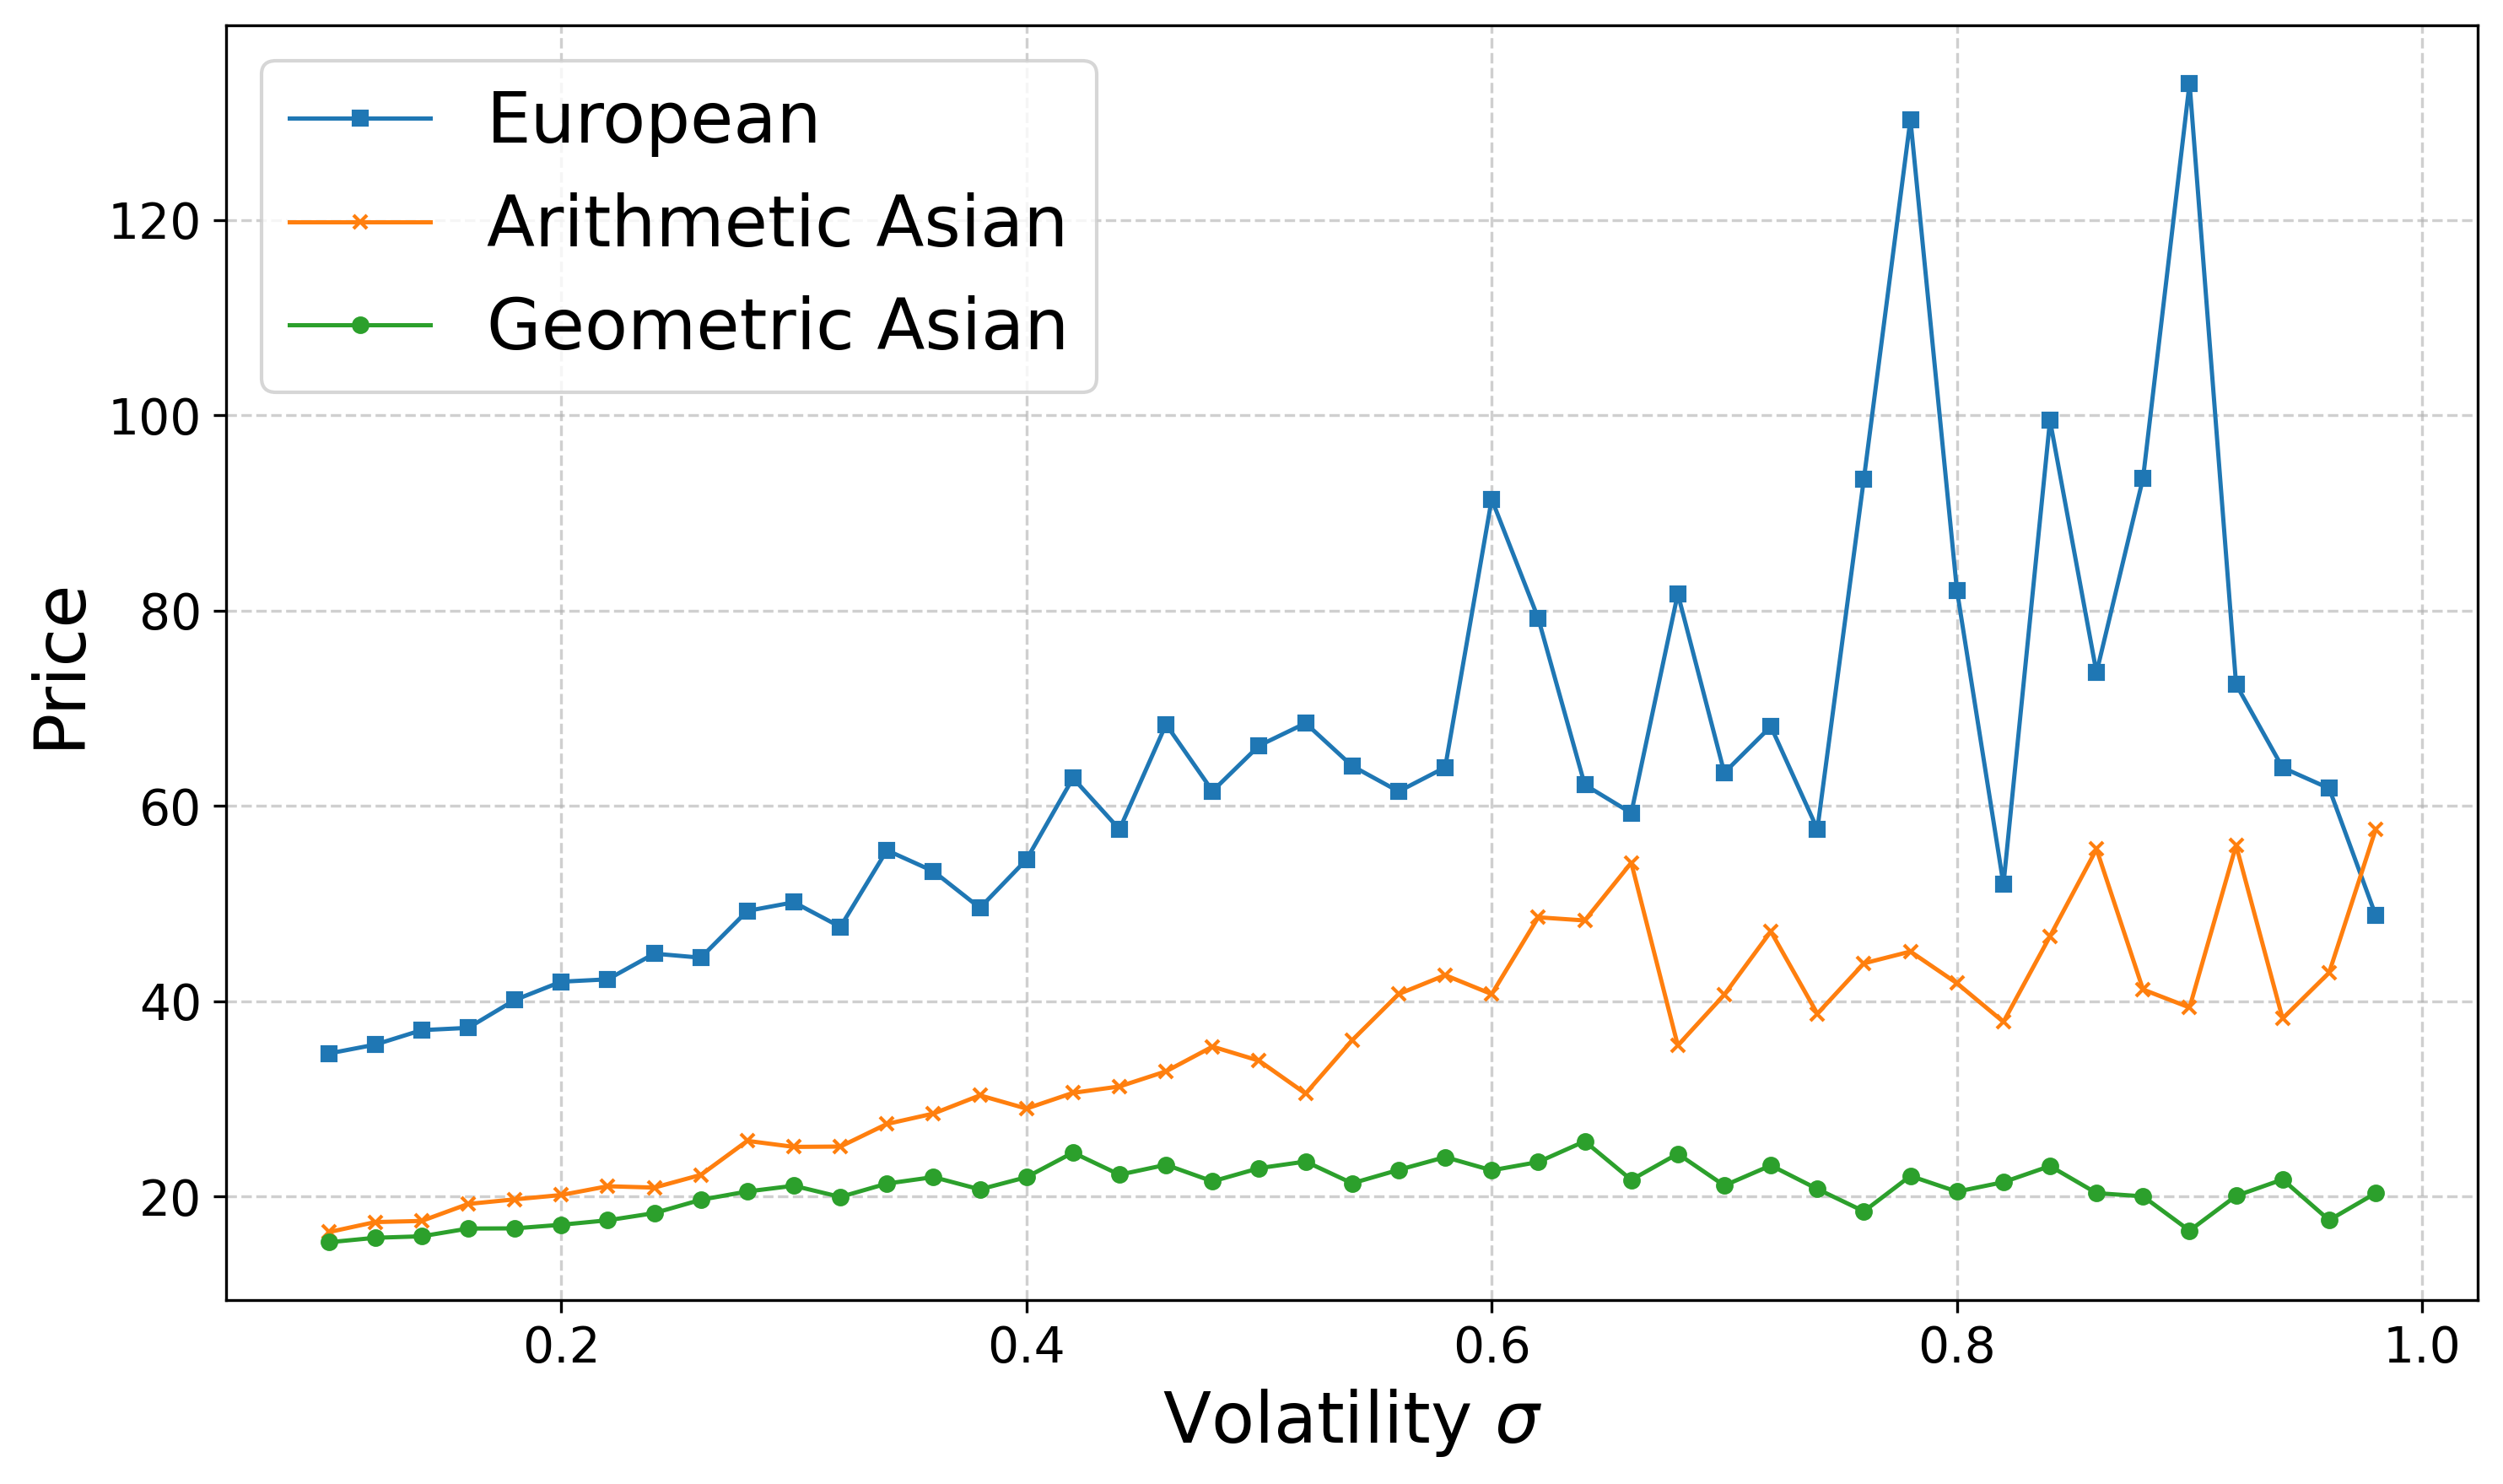
\includegraphics[width=\linewidth]{graphics/arithmetic_call_prices_sigma.png}
    \caption{Call option prices varying volatility $\sigma$.}
    \label{fig:arith_call_sigma}
\end{subfigure}
\hfill
% Bottom right
\begin{subfigure}[b]{0.45\linewidth}
    \centering
    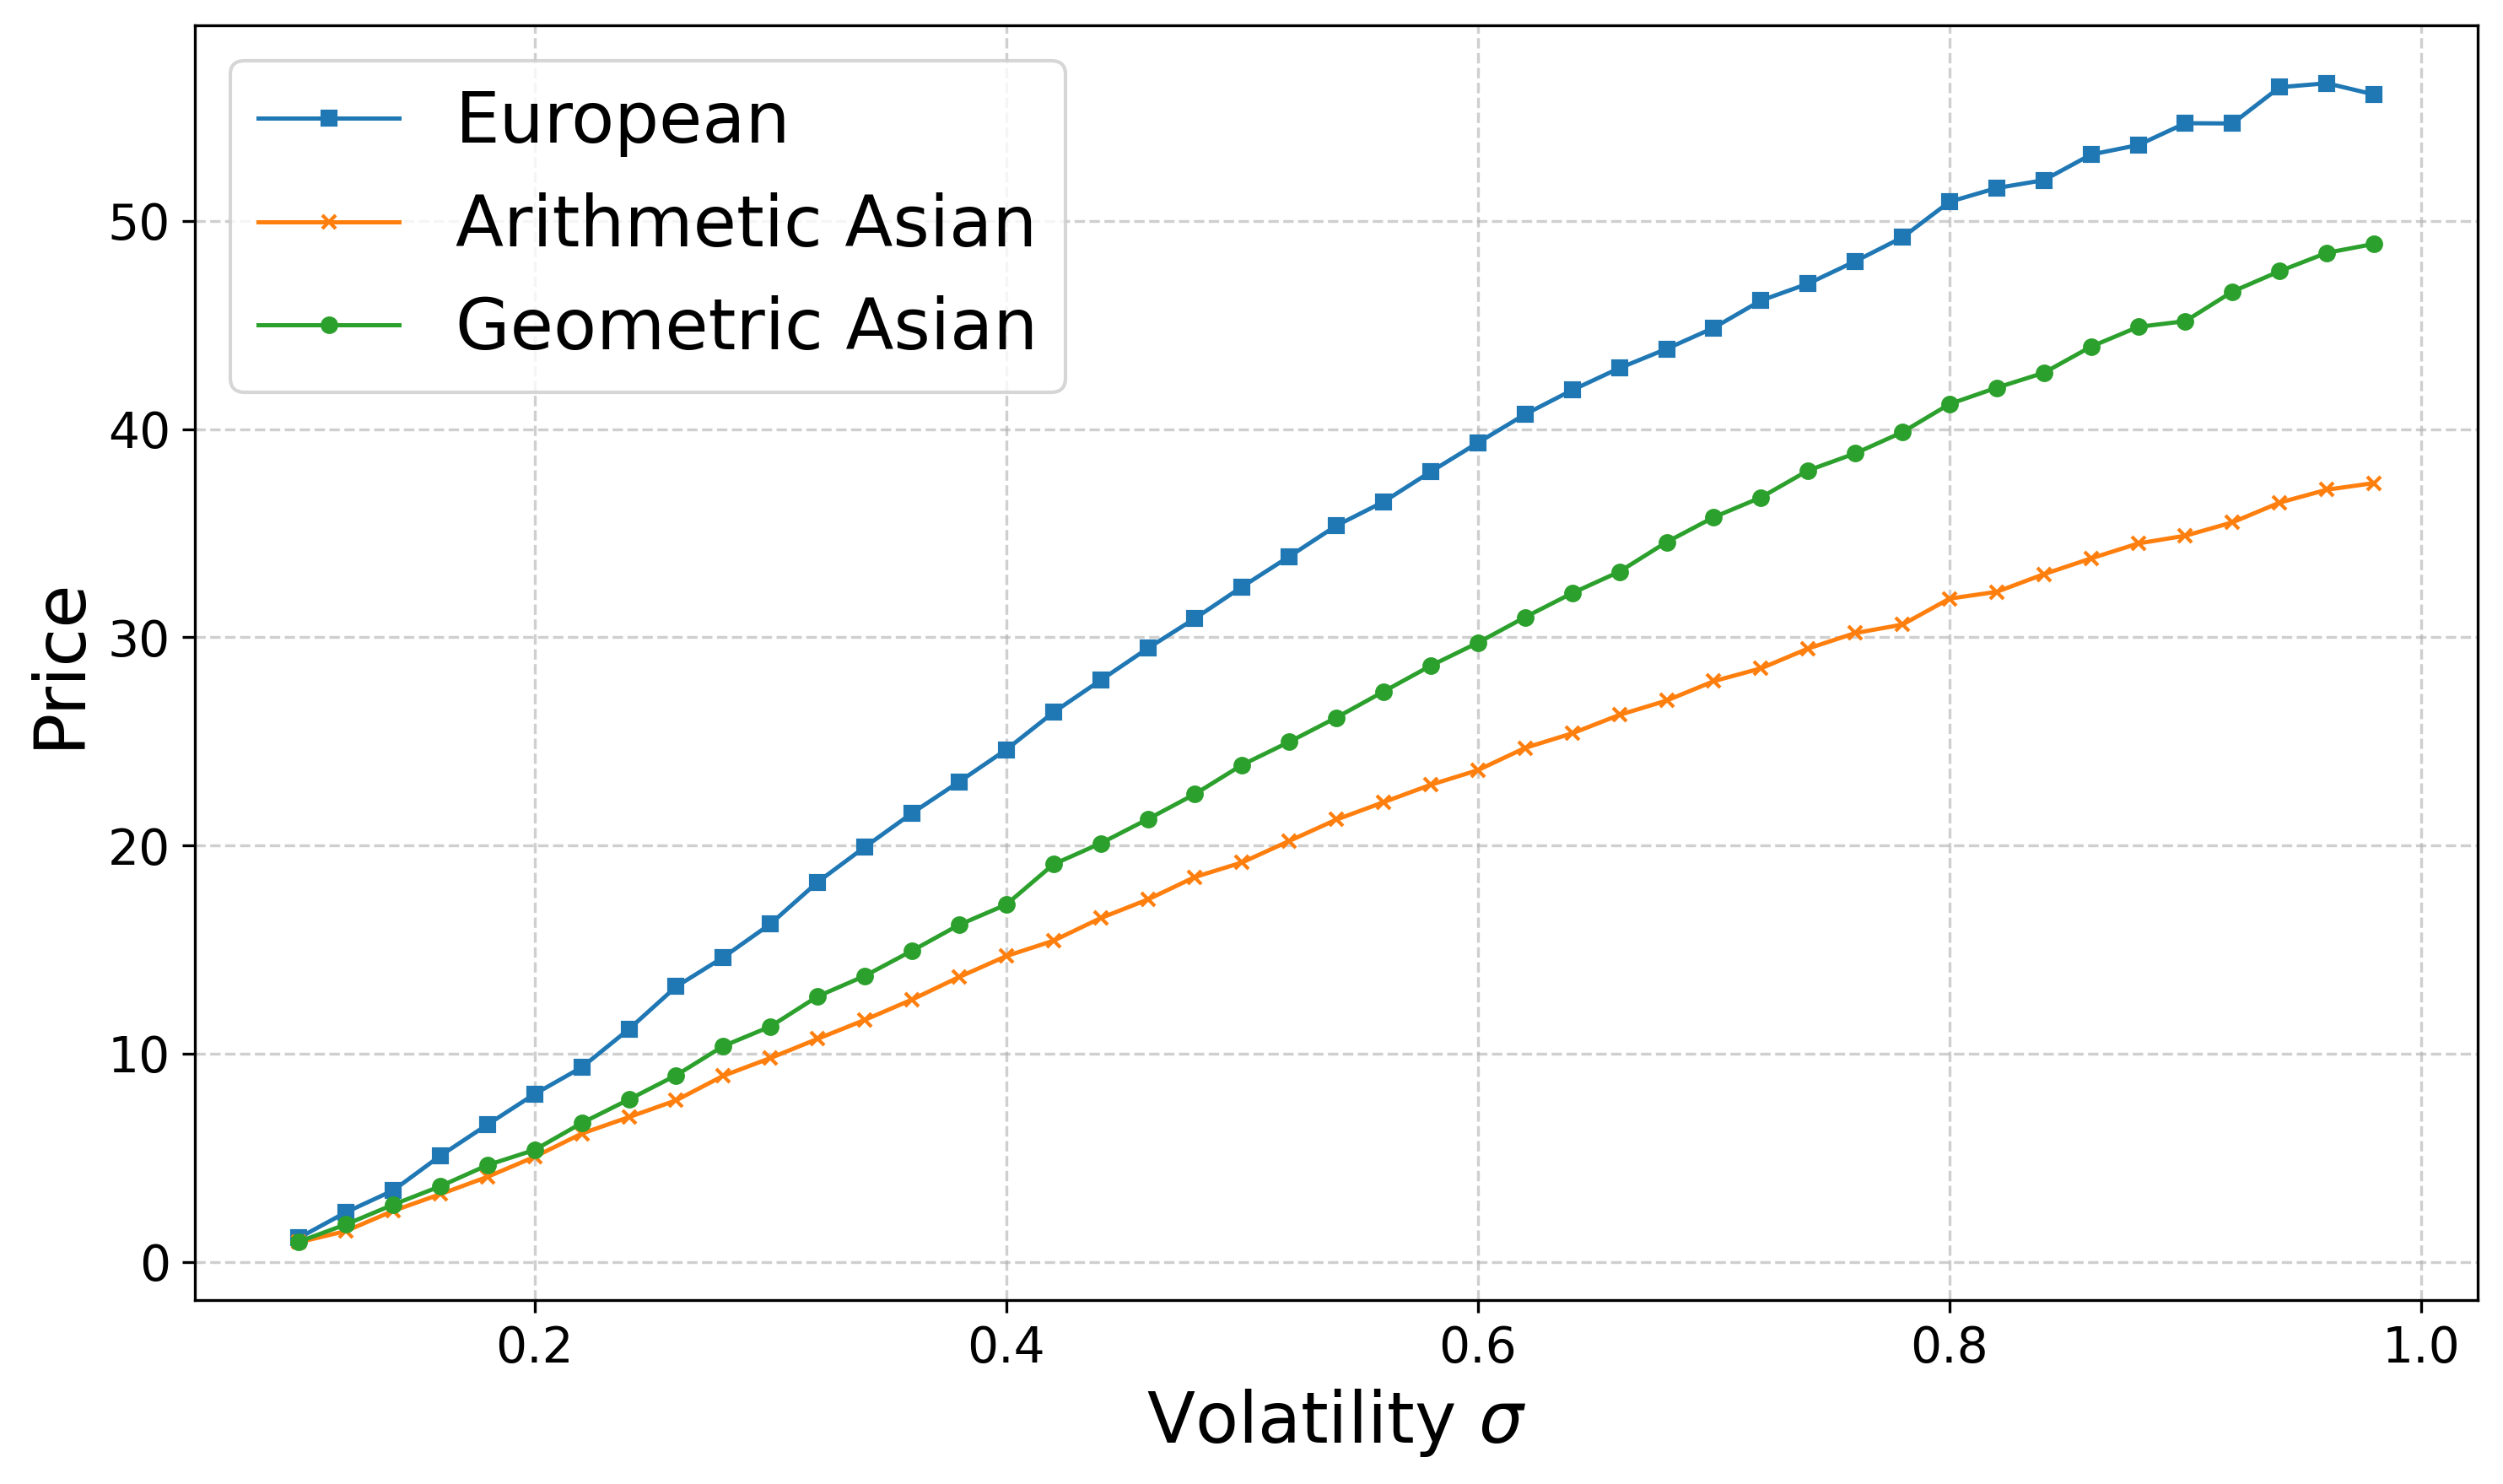
\includegraphics[width=\linewidth]{graphics/arithmetic_put_prices_sigma.png}
    \caption{Put option prices varying volatility $\sigma$.}
    \label{fig:arith_put_sigma}
\end{subfigure}

\caption{Prices obtained via Monte Carlo simulation for arithmetic Asian, geometric Asian, and European calls and puts, varying strike $K$ and volatility $\sigma$. Base parameters: $S_0 = 150$, $K=100$, $\sigma =15\%$, $T=10$, $r=4\%$, number of simulations $M=2000$, and timestep $\Delta t = \frac{T}{1000}$.}
\label{fig:asian_arith_prices}
\end{figure}

The results presented generally support the validity of our Monte Carlo approach. For call options, 
Figures \ref{fig:arith_call_k} and \ref{fig:arith_call_sigma} clearly demonstrate that the 
arithmetic Asian prices lie consistently between European and geometric Asian prices. Intuitively, 
this ordering arises because averaging reduces volatility, making Asian options cheaper than European 
options, while the geometric average provides a lower bound on the arithmetic average:
\begin{equation*}
\bar{S}_{\text{geometric}} \leq \bar{S}_{\text{arithmetic}}.
\end{equation*}
Consequently, for call payoffs, we have:
\begin{equation*}
\max(\bar{S}_{\text{geometric}} - K, 0) \leq \max(\bar{S}_{\text{arithmetic}} - K, 0).
\end{equation*}
By Jensen's inequality, since the payoff is a convex function, it follows that:
\begin{equation*}
\mathbb{E}[\max(\bar{S}_{\text{geometric}} - K, 0)] \leq \mathbb{E}[\max(\bar{S}_{\text{arithmetic}} - K, 0)].
\end{equation*}

This neatly explains why arithmetic Asian call prices consistently sit between European and 
geometric Asian call prices in our results. Similarly, this logic indicates that the geometric Asian 
put serves as an upper bound for the arithmetic Asian put, aligning with what is observed in Figures 
\ref{fig:arith_put_k} and \ref{fig:arith_put_sigma}. Figure \ref{fig:arith_put_sigma} again illustrates
that the European put option prices increase above both Asian put prices as volatility rises, consistent
with the notion that greater volatility expands potential payoffs.

Interestingly, in Figure \ref{fig:arith_put_k}, we observe that as the strike $K$ becomes large 
(approximately $K=200$ and beyond), the European put price converges with and then drops below the 
arithmetic and geometric Asian put prices. Intuitively, this could occur because, at very high strikes,
the probability of the underlying asset finishing significantly below the strike increases dramatically
for averaged payoffs compared to a single-terminal-price payoff. Hence, the Asian puts, which depend 
on the average price, can maintain higher expected payoffs in these extreme strike scenarios. We 
will investigate this intriguing behavior further in the section \ref{sec:comparison}, where we 
compare our Monte Carlo results to finite difference prices to determine whether this phenomenon is 
consistent across numerical methods.

To further improve the efficiency of our Monte Carlo estimates for arithmetic Asian options, we
now introduce the control variate technique. Control variates leverage the known analytical price 
of a closely related option to reduce variance in Monte Carlo simulations, thereby achieving lower 
standard errors.

Formally, suppose we want to estimate the expected payoff $\mathbb{E}[P(S)]$ using Monte Carlo 
simulation, and we have a related random variable $C(S)$ with a known expected value $\mathbb{E}[P(S)]$.
Then, the control variate estimator $\hat{\mu}_{cv}$ is defined as:

\begin{equation*}
\hat{\mu}_{cv} = \frac{1}{M} \sum_{i=1}^{M}\left[P(S_i) - c\left(C(S_i)-\mathbb{E}[C(S)]\right)\right],
\end{equation*}

where $c$ is chosen to minimize the variance of $\hat{\mu}_{cv}$. The optimal $c$ is given by:

\begin{equation*}
    c^* = \frac{\mathrm{Cov}(P(S), C(S))}{\mathrm{Var}(C(S))}.
\end{equation*}

In the context of arithmetic Asian options, a natural and highly effective control variate is
the geometric Asian option, since it admits a known closed-form analytic price. 
By exploiting the strong correlation between the payoffs of arithmetic 
and geometric Asian options, this choice significantly reduces the variance of our price estimates.
This approach is inspired by that taken in \cite{kemna1990pricing}. We therefore implement 
the above methodolog. The resulting effects on standard error are shown in figure:




\subsection{Finite Difference Pricing}\label{sec:FD_pricing}
\section{Comparison of Methods}\label{sec:comparison}
\section{Further work and conclusion}\label{sec:conclusion}

\printbibliography

\end{document}